\chapter{Basics}
\label{CHAPTER:BASICS}
%\label{CHAPTER:ALIGNMENT}

\section{Hidden Markov Models}
\todo{Ako to suvisi s dizertackou}
\abbreviation{Hidden Markov Models}{HMM} are graphical probabilistic models
commonly used for sequence annotation or sequence alignment. An HMM is a
probabilistic finite state machine that in every state emits one symbol. Later
we will also discuss variants of HMMs that emit more symbols or that emit
symbols on multiple tapes. In this chapter, we will describe basic definitions
and algorithms that are used with HMMs. In this thesis, we will study computational complexity of some HMM problems and we will use HMM alignment of biological sequences.

\subsection{Definitions}\label{SECTION:HMMDEF}
                       
%HMM
%Pravdepodobnost
%Posterior pravdepodobnost
%Anotacia
%Pravdepodobnost anotacie
%Footprint
HMMs are generative probabilistic models.
The generative process of an HMM starts in a random state $q$ sampled according
to the \firstUseOf{initial
distribution} $I$.  When an HMM is in some state $q$ it emits one symbol from
alphabet $\Sigma$ according distribution $e_q$ and moves to another state
according to transition distribution $a_q$. Note that emission and transition
distributions can be different for every state.  This process produces two
sequences: sequence of states $\pi=\pi_0\pi_1\pi_2\dots$ called
\firstUseOf{state path} and output sequence $X=X_0X_1X_2\dots$ over alphabet
$\Sigma$. In this work, we will use only discrete versions of HMMs with finite state
space and alphabet.  


\begin{definition}
Any square matrix $M$ of size $n\times n$ is \firstUseOf{stochastic} if it satisfies the
following properties.
\begin{enumerate}
\item $\forall 0\leq i<n,0\leq j < m, 0\leq M[i,j]\leq 1$
\item $\forall 0\le i<n, \sum_{i=0}^{m-1}M[i,j]=1$
\end{enumerate}
\end{definition}

\begin{note}
Stochastic matrix consists from $n$ probability distributions over a set of size $n$.
\end{note}

\begin{definition}\label{DEF:HMM}
A \abbreviation{Hidden Markov Model}{HMM} is a tuple $H=(\Sigma,V,I,e,a)$ where
$\Sigma=\{\sigma_0,\dots\sigma_{m-1}\}$ is a finite alphabet of size $m$,
$V=\{v_0,\dots,v_{k-1}\}$ is a finite set of state of size $k$, $I$ is
a distribution over $V$, $e$ is $k\times m$ matrix where each row contains
distribution over $\Sigma$ and $a$ is stochastic matrix of size $m\times m$.

We will index elements of $e$ and $a$ by subscripts; therefore $e_{u,v}$ is
the element in $u$-th row and $v$-th column of $e$.  

%Therefore following conditions hold:
%\begin{enumerate}
%\item $\forall v\in V, I_v \geq 0$
%\item $\sum_{v\in V}I_v=1$
%\item $\forall u\in V,\forall \sigma\in\Sigma, e_{u,\sigma}\geq0$
%\item $\forall u\in V, \sum_{\sigma\in \Sigma}e_{u,\sigma}=1$
%\item $\forall u,v\in V, a_{u,v}\geq0$
%\item $\forall u\in V, \sum_{v\in V}a_{u,v}=1$
%\end{enumerate}
\end{definition}

\begin{example}\label{EXAMPLE:EXAMPLEHMM} Consider the HMM $H=(\Sigma,V,I,e,a)$ from Figure
\ref{FIGURE:EXAMPLEHMM}.  Alphabet is $\Sigma=\{A,C,G,T\}$ and set of states is
$V=\{R,0,1\}$.  Transition and emission distributions are described in the figure.
We can define initial distribution to $I_R=0.5, I_1=0.3$ and $I_{0}=0.2$.
%Let $H=(\Sigma,V,I,e,a)$ be an HMM with
%$\Sigma=\{A,C,G,T\}$, $V={I,G}$, $I=(0.2,0.8)$,
%$e_{I,A}=0.1,e_{I,C}=0.2,e_{I,G}=0.3,e_{I,T}=0.4, e_{G,x}=0.25, x\in \Sigma$ and 
%$a_{I,I}=0.9,a_{I,G}=0.1,a_{G,G}=0.95$ and $a_{G,I}=0.05$.
\end{example}

%The conditions $1-6$ ensure that everything is correct probabilistic
%distribution.
\begin{figure}
\begin{center}
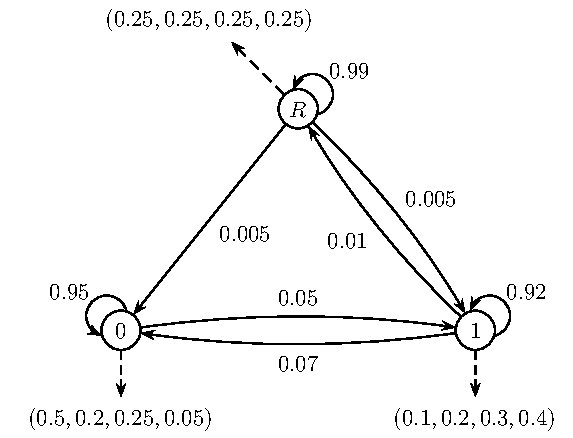
\includegraphics{../figures/exampleHMM.pdf}
\end{center}
\caption[Example of simple Hidden Markov Model]{
An HMM with $3$ states
that emits symbols from alphabet of size $4$.  Circles represents states; an arc
from state $u$ to $v$ indicates that $a_{u,v}>0$. The missing arc from state
$In$ to $R$ means that $a_{In,R}=0$. Every four tuple represents the emission distribution of the associated state.
}\label{FIGURE:EXAMPLEHMM} 
\end{figure}


\begin{definition}\label{DEF:STATEPATH}
Let $H=(\Sigma,V,I,e,a)$ be an HMM. We say that there is \firstUseOf{transition}
from state $u$ to state $v$ if $a_{u,v}>0$. We will write transition from $u$ to
$v$ as $u\to v$ and $T=\{u\to v\mid a_{u,v}>0\}$ is the set of all transitions of
$H$.

\firstUseOf{State path} $\pi=\pi_0\pi_1\dots\pi_{n-1}$ is a sequence of
states. We say that a state path $\pi$ is \firstUseOf{admissible} if $I_{\pi_0}>0$
and  $\pi_{i-1}\to\pi_i\in T$ for all $1\leq i < n$. Otherwise $\pi$ is
\firstUseOf{inadmissible}.
\end{definition}

\begin{example}
Consider the HMM from figure \ref{FIGURE:EXAMPLEHMM}. Set of transitions is
$T=\{R\to R,R\to In, R\to E,In\to In, In\to E, E\to E, E\to In, E\to R\}$.
State path $\pi_1=RRRRInER$ is an admissible state path and $\pi_2=RRRInREER$
is an inadmissible state path, because it contains a transition with zero
probability ($In\to R$).
\end{example}



%Formally, Hidden Markov Model is defined by it's finite state space
%$Q=\{q_0,q_2,\dots, q_{k-1}\}$ of size $k$, initial probabilistic distribution
%$I$ over state space, finite alphabet $\Sigma = (\sigma_0, \sigma_1, \dots,
%\sigma_{m-1})$ of
%size $m$, emission and transition distribution over $\Sigma$ and $Q$
%respectively defined for every state independently. We denote emission
%distribution of state $q$ by $e_q$ and transition distribution by $a_{q}$. 

Hidden Markov models are generative probabilistic models, meaning that they
describe a simple process that can generate a pair of state path and sequence.
In following definition we will define probability distribution of pairs (state
path, sequence) and probability distribution of sequences generated by an HMM.

\begin{definition}
Let $H=(\Sigma,V,I,e,a)$ be an HMM and $X=X_0X_1\dots X_{n-1}$ be a sequence over
alphabet $\Sigma$ of length $n$. Let $\pi$ be a state path of length $n$. Then the
probability that state path $\pi$ generated sequence $X$ is 

\[\prob{X,\pi\mid H}=
I_{\pi_0}e_{\pi_0,X_0}\prod_{i=1}^{|X|-1}a_{\pi_{i-1},\pi_i}e_{\pi_i,X_i}\]
The probability that $X$ was generated by the
model $H$ (using any state path) is 
\[\Pr\left(X\mid H\right)=\sum_{\pi\in V^n}\Pr\left(X,\pi\mid H\right)\]

\end{definition}

\begin{example}
Consider the HMM $H$ from the example \ref{EXAMPLE:EXAMPLEHMM}. Let state path be $\pi=RRInInE$ and
generated sequence be $X=ACGTT$. Then the probability that $H$ generates $\pi$
and $X$ is 
$\prob{ X,\pi\mid H } = 0.5 \cdot 0.35 \cdot 0.99 \cdot 0.25 \cdot 0.005 \cdot 0.25 \cdot 0.95 \cdot 0.05 \cdot 0.05 \cdot 0.4 =
0.5143359375  \cdot  10^{-7}$
\end{example}



\begin{note}
In our  definition of an HMM, the sum of the probabilities of all sequences of
length $n$ is $1$. Later we will discuss concept of final states. With final
states, the sum of the probabilities of all sequences (of all lengths) is one.

\end{note}

We will be interested in the three basic problems in HMMs:
\begin{enumerate}
\item Given sequence $X$ and model $H$. What is the probability that $X$ was
generated by model $H$?
\item Given sequence $X$, model $H$ and assumption that $X$ was generated by the
model
$H$, what is the best explanation of $X$? By explanation is usually meant state
path that generated $X$. We call the process of computing explanation of
sequence $X$ \firstUseOf{decoding}.
\item Given training data $D$ (usually sequences with ``explanations'') and
topology of the model (set of states and transitions), what are the best parameters
(initial, transition and emission distributions) that explains training
data $D$? This problem is also called \firstUseOf{training}
\end{enumerate} 
In following sections we will discuss several algorithms
for the problems describes above. We will mostly focus on the
decoding problem.


\subsection{The Forward Algorithm}
The Forward algorithm computes for a given sequence $X$ of
length $n$ the probability $\Pr\left(X\mid H\right)$ that the sequence was
generated by the model (it solves the first problem of HMMs) \cite{Durbin1998}. The algorithm is
based on the dynamic programming. It fills
matrix $F$ of size $n\times m$ where $m$ is the number of states of $H$, $F[i,v]$ is the probability that $H$
generated $X[:i+1]$ with state path that ends in state $v$. Values $F[i,v]$ are  called \firstUseOf{forward
variables}. $F[i,v]$ can be computed by the following equations (also called the
forward equations).

\begin{align}
F[0,v] &= I_ve_{v,X_0}, v\in V\\
F[i,v] &= \sum_{u\in V}F[i-1,u] \cdot a_{u,v} \cdot e_{v,X_i}, v\in V,0< i < n
\end{align}
%We call values $F[i,v]$ forward variables. Value $F[i,v]$ is the
%probability, that $X[:i+1]$ was generated by state path that ends with state
%$v$. 
The probability that $H$ generated $X$ is 
 \[\Pr\left(X\mid H\right) = \sum_{v\in V} F[n-1,v]\]

Using the recurrence equations above, we can compute the probability of $X$ in
$O(nm^2)$ time and $O(m)$ memory. If the transition
matrix is sparse, then this algorithm can be implemented in $O(n(m+t))$ time
where $t$ is the number of transitions.  Forward variables are also used in other
algorithms. 
%Storing all of the forward variables requires soring $O(nm)$ numbers.

\subsection{Sequence Annotation}

%definujeme annotation, footprint, set of colors

HMMs can be used for sequence annotation. By sequence annotation we mean
assigning ``labels'' to parts of the input sequence according to their meaning.
Now we give several examples of bioinformatics problems where HMMs were previously used.

\paragraph{Gene finding:} Parts of DNA sequences that are in cells translated
into proteins are called genes.  In gene finding we want to assign to every
symbol of the input sequence a gene label if it is inside a gene or a different
label if it is not part of a gene \cite{GeneWise2004, Brejova2005, Burge1997,
Alexanderson2004}. Additionally, we want to label sequence according to the
internal structure of a gene: gene starts with promoter followed by
transcription start site and ends with transcription stop site. Between
transcription sites are alternating exons and introns \cite{TODO}. 

%For example in the gene-finding domain, we want to assign gene labels to those
%parts of the sequence that encode proteins. To annotate transmembrane proteins,
%we want to know, which parts of the sequence are on which  side of the membrane.
%In recombination prediction we want to predict which parts of the sequence
%belong to which subtype of an organism.  \todo{rozviest priklady, alebo zrusit}

\paragraph{Transmembrane proteins:} Some proteins in cells pass through a membrane
from one side to the another (usually they pass through the membrane several times).  In
transmembrane protein prediction we want to assign labels to the symbols of the input
protein sequence to distinguish the parts of the sequence that are on one side of the
membrane from the parts that are on the other side of membrane or inside the membrane
\cite{Brown2010}.
%input sequence according to the side of the membrane Aim of transmembrane
%proteins is to predict which parts of the protein sequence is on which part of
%membrane and which parts are in membrane.

\paragraph{Recombination prediction:} Some organisms, for example HIV virus,
evolve rapidly and have been classified into several subtypes.  Moreover,
some viruses are mosaic combination of viruses from different subtypes. For
example, beginning and end of the sequence of a virus can be from one subtype and
the middle of the sequence is from a different subtype. In recombination prediction,
we want to annotate the sequence to distinguish between parts that originate in
different subtypes \cite{Nanasi2010,Truszkowski2011}.  

\paragraph{} In general,
we have a finite set of labels $C=\{c_0,c_1,\dots,c_{l-1}\}$ and we want to
assign one label to every symbol of the input sequence. We do it by assigning
one label to every state of an HMM.
%in a way, that states of HMM that encodes same meaning have same color. After
%that we try 
To predict the annotation of the input sequence $X$, we can  find the
most probable state path that could generate $X$ and  annotate each symbol of
the sequence $X$ according to the label assigned to the state that generated that
symbol. We can formalize it in the following definition.

\begin{definition}\label{DEFINITION:ANNOTATION}
Let $H=(\Sigma,V,I,e,a)$ be HMM and $C=\{c_0,c_1,\dots,c_{l-1}\}$ be the finite
sets of labels (or colors). Then the \firstUseOf{coloring function} 
$\lambda: V^*\to C^*$ is function that satisfies following properties:
\begin{enumerate}
\item $\lambda(v)\in C$ for all $v\in V$.
\item $\lambda(xy) = \lambda(x)\lambda(y)$ for all $x,y\in V^*$.
\end{enumerate}

Let $X$ be a sequence generated by state path $\pi$. Then annotation
$\Lambda$ of sequence $X$ is $\Lambda = \lambda(\pi)$.
\end{definition}

In the sequence annotation problem, we do not know the state path $\pi$ that
generated a given sequence. Our goal is to reconstruct the state path $\pi$ or
at least to give a good approximation of the correct annotation $\Lambda(\pi)$.
Note that in general, several state paths can have the same label.

%Since many states of the HMM can have assigned same label, there may be may be
%many state path with same annotation.

\begin{definition}
Let $H$ be an $HMM$, $X$ be a sequence of length $n$, $\Lambda$ be an annotation of sequence
$X$. The probability of annotation $\Lambda$ given sequence $X$ is 
\begin{equation}
\Pr\left(\Lambda\mid X,H\right)=\sum_{\pi \in V^n,\lambda(\pi) =
\Lambda}\Pr\left(\pi\mid X,H \right)\label{DEF:ANNOTATION:PROBABILITY}
\end{equation}
\end{definition}

Note that $\prob{\pi\mid X,H}=\frac{\prob{\pi,X\mid H}}{\prob{X\mid
H}}$.

\begin{example}\label{EXAMPLE:ANNOTATION}
Let $H$ be the HMM from the example \ref{EXAMPLE:EXAMPLEHMM}. Let $C=\{I,G\}$ and
$\lambda(R)=I$ and $\lambda(0)=\lambda(1)=G$.  Consider sequence
$X=AACT$, which was generated by the state path $\pi=R011$. The correct
annotation of $X$ is therefore  $\lambda(R011) =
IGGG$. 

 We can imagine $H$ as very simple (and not very realistic) gene
predictor. $R$ represents intergenic regions, state $In$
represents introns and $E$ represents exons. Label $I$ represents
intergenic regions and label $G$ represents regions that are genes.

Using this interpretation, the sequence $AACT$ contains gene $ACT$. There are
several state paths consistent with this annotation: if $AACT$ was generated by state path
$REEE$ then subsequence $EEE$ is exon; if it was generated by state path $REIE$
then sequence contain two exons and one intron in the middle. There are $2^3$
different state paths $\pi$ with $\lambda(\pi)=IGGG$.  All of those state path
support ``fact'' that $IGGG$ is the correct annotation of $X$.

\end{example}


%\begin{example}
%Consider again HMM from example \ref{EXAMPLE:EXAMPLEHMM} and annotation function
%from example \ref{EXAMPLE:ANNOTATION}.
%\end{example}

Given a sequence $X$, the natural question is what is the best annotation of
$X$.  One measure of quality of an annotation is its probability. The more
probable is annotation, the more likely $X$ was generated with some state path with
such annotation. We can formulate this in following problem.

\begin{definition}
Given HMM $H$ and sequence $X$, \abbreviation{the most probable annotation
problem}{MPA} is the problem of finding an annotation $\Lambda$ of $X$ that maximizes
the probability \[\prob{\Lambda\mid X,H}\]
\end{definition}

\begin{theorem}
Most probable annotation problem is NP-hard.
\end{theorem}
This theorem was proved in 2002 by Lyngsø {\it et al.} and proof can be found in
\cite{Lyngso2002}. Their proof was done by a reduction from the maximum clique problem.
For input graph with $n$ vertices they construct an HMM $H$ with $O(n^2)$ states and
sequence $X$ of the length $n$. The most probable annotation of $X$ could be
converted into maximum clique of input graph. 
Their result was later strengthened in a sense that the problen is hard even for some constant-sized HMMs \cite{Brejova2007mpa}.

\begin{theorem}
There exists an HMM such that it is NP-hard to find the most probable annotation
to a given input sequence $X$.
\end{theorem}
\todo{Presunut za Viterbiho?}
This paper also
contain polynomial algorithm (Extended Viterbi Algorithm) that finds most
probable annotation for special classes of HMMs. 

Note that from the probabilistic nature of the HMMs, the most probable
annotation does not have to be the best approximation of the correct annotation.
We will discuss alternative decoding criteria in section \ref{TODO}.
\nocite{Brown2010,Gross2007,Nanasi2010,Truszkowski2011}.

\subsection{The Viterbi Algorithm}
%\todo{Viterbi variable ma rovnake oznacenie ako mnozina stavov. Treba to
%upravit} -- Brona tvrdi ze netreba
\todo{Zle nadvazuje na anotaciu. Mozno dat pred anotaciu?}
The Viterbi algorithm  is probably the most frequently used
decoding algorithm for hidden Markov
models \cite{Durbin1998}.
The Viterbi algorithm answers a straightforward question: given the sequence
$X=X_0X_1\dots X_{n-1}$, what
is the most-likely state path $\pi$ that generates $X$? Formally, Viterbi
algorithm finds a state path maximizing $\Pr\left( \pi\mid X,H \right)$. Since
\[\Pr\left(\pi\mid X,H\right) = \frac{\Pr\left(\pi,X,\mid
H\right)}{\Pr\left(X\mid H\right)}\] and quantity $\Pr\left(X\mid H\right)$ is
fixed, the most probable state path $\pi$ also maximizes $\Pr\left(X,\pi\mid H\right)$. 

The Viterbi algorithm is very similar to the  Forward algorithm. It starts with computing
Viterbi variables $V[i,v]$. Variable $V[i,v]$ stores the probability of the most probable 
state path that generated $X[:i+1]$ and ends in state $v$. The algorithm
also computes back-links $B[i,v]$ that contain the previous state in the most
probable state path that generated $X[:i+1]$ and ends in state $v$. We can
compute these values by the following equations (called the Viterbi equations):
\begin{align}
V[0,v] &= I_{v}e_{v,X_0}, v\in V\\
V[i,v] &= \max_{u\in V} V[i-1,u]a_{u,v}e_{v,X_i}, v\in V,0<i<n\\
B[i,v] &= \arg\max_{u\in V} V[i-1,u]a_{u,v}e_{v,X_i}, v\in V,0<i<n
\end{align}
\begin{note}
Values $B[0,v],v\in V$ are not needed in the algorithm.

Note the similarity of the Viterbi algorithm and the Forward algorithm.
We can obtain the Viterbi equations from the Forward equations by replacing
summation with
maximization.
\end{note}


Variable $V[n-1,v]$ contains the probability of the most probable state path
that generated $X$ and ends in state $v$. Therefore the state $v_{\max} =
\arg\max_{v\in V}V[n-1,v]$ is the last state of the most probable state path.
Variable $B[n-1,v_{\max}]$ contains the previous state of the most probable
state path. By traversing back through back-links $B$ we can reconstruct the most
probable state path in $O(n)$ time.

Time complexity of the Viterbi algorithm is $O(nm^2)$ or $O(n(m+t))$ for sparse
transition matrices ($m$ is the number of states and $t$ is the number of
transitions).


We can use the Viterbi algorithm to annotate sequence $X$ by finding the most
probable state path $\pi$ and then computing $\lambda(\pi)$. If the  coloring
function $\lambda$ is the identity function, this will find the most probable
annotation, but in general the Viterbi algorithm is not even a good approximation of
the most probable annotation as shown in the following example.

\begin{figure}
\begin{center}
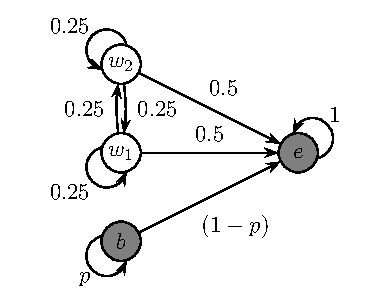
\includegraphics{../figures/multiplePathProblemHMM.pdf}
\end{center}
\caption[Hidden Markov Model with multiple path problem.]{Example of an HMM with
multiple path problem. States $w_1,w_2,b$ emit symbol $0$ with probability $1$
and state $e$ emits symbol $1$ with probability $1$. Initial distribution is set
to $I_{w_1}=I_{w_2}=\frac14, I_{b}=0.5$
and $I_e=0$. Annotations of the states are represented by the colors of the states
($\lambda(w_1)=\lambda(w_2)$ and $\lambda(b)=\lambda(e)$). }\label{FIGURE:BADVITERBIEXAMPLE}
\end{figure}

\begin{example} \todo{Pouzivamie niekde multiple path problem?}
Consider the HMM from Figure \ref{FIGURE:BADVITERBIEXAMPLE}. Take sequence
$X=0^n1$.  Since state $e$ is the only state that can emit $1$, every state
path with non-zero probability ends in state $e$. If a state path starts in
state $b$ then state path has form $b^ne$. Annotation of such a state path is
$\Lambda_1=\lambda(b)^{n+1}$ and probability of the annotation $\Lambda_1$ (and
also the state path $b^ne$) is $p^n(1-p)$.  If a state path starts in the one
of the white states, then a state path has form $w'_0w'_1\dots w'_{n-1}e$ where
$w'_i$ is either $w_1$ or $w_2$.  There are $2^n$ such state paths and each of
them has probability $0.5\cdot 0.25^n$ and annotation
$\Lambda_2=\lambda(w_1)^n\lambda(e)$. Probability of annotation $\Lambda_2$ is
therefore $0.5^{n+1}$.  If $n$ is sufficiently high and $\frac14<p<\frac12$
then the most probable state path is $b^ne$ which corresponds to the annotation
$\Lambda_1$. However, the most probable annotation is $\Lambda_2$ and its
probability is exponentially higher then the probability of $\Lambda_1$.
Therefore the Viterbi algorithm it not even a good approximation of the most
probable annotation problem.

\begin{comment}
We say that an HMM has the \firstUseOf{multiple path problem} if it has an annotation that
corresponds to more than one state path.
\end{comment}
\end{example}


\subsection{The Forward-Backward Algorithm and  the Posterior Decoding}

The \firstUseOf{Posterior decoding} is another commonly used decoding method
\cite{Kall2005, Durbin1998}. In contrast to the Viterbi algorithm, the
Posterior decoding assigns a label individually to every symbol of an input
sequence and does not care about the overall structure of the reconstructed
state path. 

Given sequence $X$, posterior decoding finds state path $\pi$ with the following
property:
\[\forall 0\leq i< n, \pi_i=\arg\max_{v\in V}\Pr\left(\pi_i=v\mid X,H\right) \]
where \[\Pr\left(\pi_i=v\mid X,H\right) = \sum_{\pi\in V^n,\pi_i=v}\Pr\left(\pi\mid X,H\right)\]

Values $\Pr\left(\pi_i=v\mid X,H\right)$ for every
combination of position $i$ and state $v$ can be computed using the Forward-Backward
algorithm. In particular,

\begin{equation}
\Pr\left(\pi_i=v,X\mid H\right) =  F[i,v]B[i, v]
\end{equation}
In this formula, value $B[i, v]$ is defined as 
\begin{equation}
B[i, v] =	
					\sum_{\pi\in V^{n-i},\pi_0=v}
					\prod_{j=1}^{n-i-1} e_{\pi_j,X_{i+j}}a_{\pi_{j-1},\pi_j}
\end{equation}
\begin{comment}
We derive the formula for efficient computation of the  $\Pr\left(\pi_i=v\mid
X,H\right)$.
\begin{align}
\Pr\left(\pi_i=v,X\mid H\right) &=  
%\sum_{\pi\in V^n,\pi_i=v}\Pr\left(\pi\mid X,H\right)
%					\label{PosteriorDer1} \\
%				&=& 
				\sum_{\pi\in
				V^n,\pi_i=v}I_{\pi_0}e_{\pi_0,X_0}\prod_{j=1}^{n-1}e_{\pi_j,X_j}a_{\pi_{j-1},\pi_j}
					\label{PosteriorDer2}\\
%				&= \sum_{\pi\in V^n,\pi_i=v}I_{\pi_0}e_{\pi_0,X_0}
%				\left( 
%					\prod_{j=1}^{i-1} e_{\pi_j,X_j}a_{\pi_{j-1},\pi_j}
%				\right)
%				a_{\pi_{i-1},\pi_i}e_{\pi_i,X_i}
%				\left(  
%					\prod_{j=i+1}^{n-1} e_{\pi_j,X_j}a_{\pi_{j-1},\pi_j}
%				\right)
%					\label{PosteriorDer3}\\
				&= \sum_{\pi\in V^n,\pi_i=v}I_{\pi_0}e_{\pi_0,X_0}
				\left( 
					\prod_{j=1}^{i-1} e_{\pi_j,X_j}a_{\pi_{j-1},\pi_j}
				\right)
				a_{\pi_{i-1},v}e_{v,X_i}
				\left(  
					\prod_{j=i+1}^{n-1} e_{\pi_j,X_j}a_{\pi_{j-1},\pi_j}
				\right)
					\label{PosteriorDer4}\\
				&= 
				\left(
					\sum_{\pi\in V^{i+1},\pi_i=v}I_{\pi_0}e_{\pi_0,X_0}
					\left(
						\prod_{j=1}^{i} e_{\pi_j,X_j}a_{\pi_{j-1},\pi_j}
					\right)
				\right)
				\left( 
					\sum_{\pi\in V^{n-i},\pi_0=v}
					\prod_{j=1}^{n-i-1} e_{\pi_j,X_{j+i}}a_{\pi_{j-1},\pi_j}
				\right)
					\label{PosteriorDer5}\\
				&= F[i,v]
				\left( 
					\sum_{\pi\in V^{n-i},\pi_0=v}
					\prod_{j=1}^{n-i-1} e_{\pi_j,X_{i+j}}a_{\pi_{j-1},\pi_j}
				\right)
					\label{PosteriorDer6}
\end{align}
The right part of the formula \ref{PosteriorDer6} has
similar structure as $F[i,v]$, but it uses last part of the state path and
sequence and also it lack initial distribution.
\end{comment}

We can compute 
these values using  the Backward algorithm, which is very similar to the Forward
algorithm. 
\begin{align}
B[i,v]&=
%\sum_{\pi\in V^{n-i},\pi_0=v}
%	\prod_{j=1}^{n-i-1}
%		e_{\pi_j,X_{i+j}}a_{\pi_{j-1},\pi_j}\\
% &= 
% \sum_{u\in V}
% 	e_{u,X_{I+1}}A_{V,u}
%	\sum_{\pi\in V^{n-i-1},\pi_0=u}
%		\prod_{j=1}^{n-i-2}
%			e_{\pi_j,X_{i+j+1}}a_{\pi_{j-1},\pi_j}\\
% &= 
\begin{cases}
1 & \textrm{if $i=n-1$}\\
 \sum_{u\in V}
 	e_{\pi_j,X_{i+1}}a_{v,u}B[i+1,u] & \textrm{otherwise}
\end{cases}
\end{align}

\begin{comment}
If we set $B[n-1,v]$ to $1$, we have a recurrence to compute values
$B[i,v]$. This recurrence is very similar to recurrence $F[i,b]$. Recall that
\[F[i,v] = \sum_{u\in V}F[i-1,u] a_{u,v} e_{v,X_i}\]
\end{comment}
The cell $B[i,v]$ depends on the next positions in sequence $X$,
while $F[i,v]$ depends on the previous positions in sequence $X$. Another
difference is that $B[i,v]$ does include emission of $X[i]$ while $F[i,v]$ does.

\begin{comment}
In addition, it is possible to compute probability
of $X$ being generated by the model with backward algorithm.

\begin{align}
\prob{X\mid H} &= 
	\sum_{\pi\in V^n}
		e_{\pi_0,X_0}\prod_{i=1}^{n-1}e_{\pi_i,X_i}a_{\pi_{i-1},\pi_i}\\
	&=
	\sum_{u\in V}e_{u,X_0}
	\sum_{\pi\in V^n,\pi_0=u}
		\prod_{i=1}^{n-1}e_{\pi_i,X_i}a_{\pi_{i-1},\pi_i}\\
	&=
	\sum_{u\in V}e_{u,X_0}B[0,u]
\end{align}

Posterior probabilities can be computed by
\[\Pr\left(\pi_i=v\mid X,H\right) = \frac{F[i,v]\cdot B[i,v]}{\Pr\left( X\mid H
 \right)}\]
\end{comment}

We can compute values of $F[i,v]$ and $B[i,v]$ and find the posterior decoding
in $O(n(m+t))$ time and $O(nm)$ memory.  Advantage of posterior decoding is
that it uses information from many slightly suboptimal state paths as opposed
to Viterbi decoding, which uses only one state path. One drawback is that it
can reconstruct inadmissible state path. One example is given below.



\begin{figure}
\begin{center}
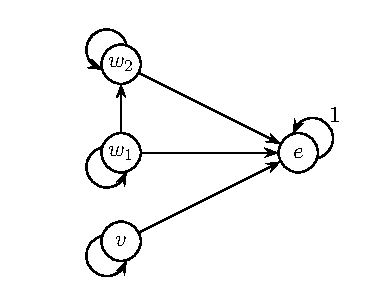
\includegraphics{../figures/posteriorInadmissibleStatePath.pdf}
\end{center}
\caption[Hidden Markov Model on which posterior decoding reconstructs
inadmissible state path]{
Example of an HMM on which the Posterior decoding reconstructs inadmissible state path. 
All unlabeled transitions are even ($0.5$). States $w_1,w_2,$ and $v$ emits $0$
with probability $1$ and state $e$ emits $1$ with probability $1$.
Initial distribution is set to $I_{w_1}=I_{w_2}=0.3, I_{v}=0.4, I_{e}=0$.
}\label{FIGURE:INADMISSIBLESTATEPATH}
\end{figure}

%\todo{Je mozne, ze by sa TU mohlo spomenut a maximalizacii ocakavaneho poctu
%spravne predikovanych stavov}

\begin{example}
Consider an HMM from figure \ref{FIGURE:INADMISSIBLESTATEPATH}. Let $X=001$. There
are three state paths that have non-zero probability:
$\pi_1=w_1w_2e,\pi_2=w_2w_1e,$ and $\pi_3=vve$. Their probabilities are
$\prob{\pi_1\mid X,H}=\prob{\pi_2\mid X,H}=0.3,$ and $\prob{\pi_3\mid X,H}=0.4$
respectively.
Posterior probabilities are in table \ref{TABLE:INADMISSIBLESTATEPATH}.
As we can see, the maximal posterior probability for the first position has state
$v$. For the second position it is state $w_2$ and for the third it is state
$e$. Therefore PD will reconstruct state path $vw_2e$. However, this state path 
is inadmissible since  $v\to w_2$ is not a transition (it has zero probability).

\begin{table}
\begin{center}
\begin{tabular}{|l|c|c|c|}
\hline
State/Position & $X_0$ & $X_1$ & $X_2$ \\\hline
$w_1$ & $0.3$ & $0$ & $0$ \\\hline
$w_2$ & $0.3$ & $0.6$ & $0$ \\\hline
$v$   & $0.4$ & $0.4$ & $0$\\\hline
$e$  & $0$ & $0$ & $1$ \\\hline
\end{tabular}
\end{center}
\caption[Example of posterior probabilities.]{Posterior probabilities for
the sequence $X$ and the HMM $H$ from the figure \ref{FIGURE:INADMISSIBLESTATEPATH}.
}\label{TABLE:INADMISSIBLESTATEPATH}
\end{table}

\end{example}


\subsection{Training} 

Training is the process of estimating parameters of the probabilistic models. In this
section we briefly describe several approaches for estimating transition and
emission distributions of hidden Markov models.

We use the \firstUseOf{maximum likelihood approach}. Let $H_{\theta}$ be an HMM
where $\theta$ contains emission and transition probabilities and
let $D$ be training data (the set of pairs $(X,\pi)$ where $X$ is sequence and $\pi$ is a state path).  We
want to find $\theta$ that maximizes the likelihood of the data:

\[L(H_\theta\mid D)=\prob{D\mid H_\theta}= \prod_{(X,\pi)\in D}\prob{X,\pi\mid H_\theta}\]

Under this scenario, we can use the frequencies of occurred events as the parameters of the model \cite{Durbin1998}.
Let $A_{u,v}$ be the number of transitions from $u$ to $v$ in $D$.
Let $E_{u,x}$ be the number times when state $u$ emitted $x$ in training data
$D$.
Then 
\begin{align*}
&a_{u,v}=\frac{A_{u,v}}{\sum_{w\in V}A_{u,w}}
&e_{u,x}=\frac{E_{u,x}}{\sum_{y\in\Sigma}E_{y,x}}
\end{align*}
for all $u,v\in V, x\in\Sigma$. Parameters $\theta=(e,a)$ maximize the likelihood
\cite{Durbin1998}. If case of insufficient data, some events that have
nonzero probability may not occur in the data and therefore their probability will be
estimated to zero. To avoid this behavior, we can use pseudo-counts
\cite{Durbin1998}: we artificially add a constant $k_x$ to the counts of all
events $x$ that we expect to have non-zero probability.

\subsubsection{Training with Missing Data} 
In case that some data are missing (for example a part
of the state path or part of the sequence) we treat the missing data as random
variables. We can use the following algorithm. 
\begin{enumerate}
\item  Set the initial parameters $\theta_0$. Let $i=0$
\item  Using model $H_{\theta_i}$, compute the expected number of occurrences of
all events (the values $A_{u,v}, E_{u,x}, u,v\in V,x\in\Sigma$). Compute the new
parameter set $\theta_{i+1}$ from the expected counts (using the method
described above). Set $i=i+1$.
\item If stopping criterion was not reached, go to step two. Otherwise 
set the $H_{\theta_{i}}$ as the final model.
\end{enumerate}
This algorithm is called the Baum-Welch algorithm and it is an instance of the
more general Expectation maximization algorithm \cite{Durbin1998}. Sequence $\{L(H_{\theta_i}\mid D)\}_{i\geq 0}$ is non-decreasing and
 converges to a local minimum \cite{Durbin1998}. As a stopping criterion,
we can use the number of iterations or the change in the likelihood.
 The expectations of the number of events can be
computed by a variant of the Forward-Backward algorithm.

In step $2$ we can replace the Forward-Backward algorithm with the Viterbi
algorithm. In such case the Viterbi algorithm computes the most probable values
for the missing data and new model is estimated from this data.
This approach is called the Viterbi training.  While the Viterbi training does
not have to converge to local maxima, it is faster in practice
\cite{Durbin1998}.  In practice we can use the Viterbi training for the
estimation of good starting parameters for the Baum-Welsch training. The
approach was used in \cite{FEAST2011}.

\subsection{Variants of Hidden Markov Models}

In this section we describe several variants of hidden Markov models.  Some of
these extensions have more expressive power but mostly they are introduced for
simplifying  models. We will use all the described variants later in the
thesis.

\subsubsection{Silent states}

One common variant of HMMs are HMMs with silent states. A silent state is a state
that does not emit any symbol. In the presence of silent states a state path can
be longer than the emitted sequence. However, the number of non-silent states in
the state path has to be equal to the sequence length. Silent states do not
add any expressive power to HMMs, but in some cases they allow to reduce the
number of transitions by a factor $m$. This can be used to decrease the number of
parameters and speed up algorithms. 

\begin{comment}
\begin{definition}
Hidden Markov Model with silent states is a
tuple $H=(\Sigma,V,Q,I,e,a)$
where $\Sigma,V,I,a$ are defined as in definition \ref{DEF:HMM}. $Q\subseteq V$ is set of
silent states. $e$ must satisfy the following conditions:
\begin{enumerate}
\item $\forall u\in V\backslash Q,\forall \sigma\in\Sigma, e_{u,\sigma}\geq0$
\item $\forall u\in Q,\forall \sigma\in\Sigma, e_{u,\sigma}=0$
\item $\forall u\in V\backslash Q, \sum_{\sigma\in \Sigma}e_{u,\sigma}=1$
\end{enumerate}
\end{definition}

\begin{definition}
Transitions and state path are defined as in definition \ref{DEF:STATEPATH}. 

Let $\pi$ be a state path. \firstUseOf{Non-silent state path} $\pi^Q$ is
the maximal subsequence of $\pi$ that consists of non-silent states.
\end{definition}

\begin{note}
Non-silent state path $\pi^Q$ can by obtained from a state path $\pi$ by removing all silent
states.
\end{note}

\begin{definition}
Let $H=(\Sigma,V,Q,I,e,a)$ be an HMM with silent states and $X=X_0X_1\dots
X_{n-1}$ be a sequence over
alphabet $\Sigma$ of length $n$. Let $\pi$ be a state path for which $\pi^Q$ has
length $n$. Then the probability that state path generated sequence $X$ is 

\[\Pr\left(X,\pi\mid H\right) =
I_{\pi_0}\left(\prod_{i=1}^{|\pi|-1}a_{\pi_{i-1},\pi_i}\right)\left(\prod_{i=0}^{|X|-1}e_{\pi^Q_i,X_i}\right)\]

If length of the sequence $X$ is not equal to the length of the non-silent state
path $\pi^Q$, then the
probability that $\pi$ generates $X$ is zero.
\end{definition}
\end{comment}

\begin{example}
Example of an HMM with silent states that reduces the number of transitions by factor
of $\Theta(m)$.
\todo{Prepis tento example na profilove HMM}

Consider following HMM $H=(\Sigma,V,I,e,a)$ with $m$ states such that every row
of $a$ is the uniform distribution over $V$. In other words, there is transition
between any two pairs of states from $V$, that is exactly $n^2$
transitions\footnote{$u\to u$ is also a transition}.

We create a new HMM $H'$ by removing all transitions from $H$, adding one silent
state $s$ and adding transitions
from state $s$ to all states from $V$ with probability $\frac1m$  and from every
state $V$ to $s$ with probability $1$. This new HMM
defines the same distribution of sequences, but has one more state and only $2m$
transitions. 

The Viterbi algorithm, the Forward algorithm or Posterior decoding can be
implemented for $H'$ in $O(nm)$ time while these algorithm will have time
complexity $O(nm^2)$ for $H$.
\end{example}

There should not be the cycle from transitions between silent states, because
it causes problems with the order of computations of the Viterbi algorithm, the
Forward algorithm and others. For example if we have silent cycle out of states
$u$ and $v$, the recurrency for computing the Forward algorithm contain a
cycle: value $F[i, v]$ depends on value $F[i, u]$, and value $F[i,u]$ depends
on value $F[i, v]$.  Such cycles can be removed from an HMM without affecting
of the distribution of the sequence. Additionally, for every HMM with silent
states there is an HMM without silent states that defines same distribution of
sequences \cite{Nanasi2010mgr}.


\subsubsection{Start and Final state}

Sometimes it is useful to have a special start state and a special final state.
Start states can be used instead of the initial distribution. State $s$ is a start
state, if $I_v=1$. Conversely, we can model arbitrary initial distribution by a silent start state $s$
with $a_{s,v}=I_v$ for all $v$.

In contrast, final states affect distribution of the model. An HMM defined in section
\ref{SECTION:HMMDEF} defines a distribution over the sequences of the same length.
An HMM with
final states defines distribution over sequences of all lengths.  We denote the
set of final states $F\subseteq V$. Transitions from final states are not
defined (or set to zero). Emission distribution might be defined (if not, final
states are silent). Every state path has to end with a final state, and
final state can be only at the end of a state path.

With final states, HMM stops generating a sequence once it reaches some final
state. Therefore the sum of the probabilities of all sequences is $1$.

Final states slightly affect algorithms. For example in the Forward algorithm
we do not have to change recurrences, only the final summation: probability of
the sequence is $\sum_{q\in F}F[n-1,q]$.  Similarly, in the Viterbi algorithm
we have to find $\max_{q\in F} V[n-1,q]$ not $\max_{q\in V} V[n-1,q]$.  The
Backward algorithm is changed by setting $B[n-1,q]$ to zero for all $q\notin
F$.

\subsubsection{High Order HMMs}

Sequence $X$ and a state path $\pi$ generated by an HMM can by considered as
sequences of random variables $X_0,X_1,\dots, X_{n-1}$ and
$\pi_0,\pi_1,\dots,\pi_{n-1}$.  Random variables associated with the state path
have the Markov property \cite{Levin2006}, which means that $\pi_i$ depends
only on $\pi_{i-1}$ or more precisely
$\prob{\pi_i\mid\pi_0,\dots,\pi_{i-1}}=\prob{\pi_i\mid\pi_{i-1}}$. Similarly,
$X_i$ depends only on $\pi_i$, that is
$\prob{X_i\mid\pi_0,\dots,\pi_i,X_0,\dots,X_{i-1}}=\prob{X_i\mid\pi_i}$.
However, sometimes the  ability to look back more than just one state or symbol
is useful. We can extend the transition and the emission probabilities to
depend on several previous states/emissions. 

\begin{comment}
It is possible to depend on whole previous
sequence, however it increase running time of decoding and training algorithms.
If we depend only on all previous emissions, time complexity of such algorithm
will increase by factor of $n$. If we depend on all previous state paths then
time complexity of those algorithms can increase exponentially.  Therefore
practical solutions that are using high-order HMM depends only on small number
of previous states/emissions .
\end{comment}

\nocite{Brejova2005,Alexanderson2004}
We will briefly discuss $k$-th order HMMs where emissions are dependent on
previous $k$ emissions. Specifically, $X_i$ depends only on $\pi_i$ and
$X_{i-k},\dots,X_{i-1}$. Emission distribution is therefore parametrized by
state and previous emissions, which is a string of length at most $k$ (it can be
shorter in the beginning of the sequence). $e_{u,x,a}$ is probability that
state $u$ emits $a$ under the condition that $x$ is the suffix of the already emitted
sequence. Let $X$ be sequence and $\pi$ be state path. Then definition
of probability that $X$ and $\pi$ were generated by the model changes to

\[
\prob{X,\pi\mid H} = 
I_{\pi_0}e_{\pi,\varepsilon,X_0}\prod_{i=1}^{n-1}
e_{\pi_i,X[i-\min\{k,i\}:i],X_i}a_{\pi_{i-1},\pi_i}
\]
where $\varepsilon$ is empty string. Other definitions will not change. We can
use all algorithms that we have described above, but we have incorporate these
new emission distributions.

\subsubsection{Generalized HMMs}

Consider a state $v$ with a self-transition, i.e. a state for which $e_{v,v}>0$.
The number of steps the model remains in this state is distributed according to
the geometric distribution.
In particular, the probability that we will leave state $v$ after exactly $k$ steps is
$e_{v,v}^{k-1}(1-e_{v,v})$. For some
applications this behaviour not
appropriate \cite{Burge1997,Majoros2004}.

A \abbreviation{generalized hidden Markov model}{GHMM} (or hidden semi-Markov model)
has with every state $v$ associated a duration distribution $d_v$.  When
a GHMM enters state $v$, it first samples length $l$ according
to the distribution $d_v$.  Afterwards it generates string $x$ of length $l$.  To
specify the probability $e_{v,x}$, each symbol of generated string $x$ is usually
generated independently, which means that $e_{v,x}=\prod_{i=0}^{|x|-1}e_{v,x[i]}$.
Output of a GHMM are three sequences: state path $\pi=\pi_0\pi_1\dots\pi_{l-1}$,
\firstUseOf{duration sequence} $D=D_0D_1\dots D_{l-1}$ and sequence
$X=X_0X_1\dots X_{n-1}$.  The state path and the duration sequence has same
length and \[\sum_{i=0}^{|D|-1}D_i = |X|\].

Manipulation with GHMMs is  more complicated and technical.
\begin{comment}
If one state can
generate strings with various lengths then in general, from state space we are
not able to uniquely assign to symbols of a sequence $X$ the state which 
generated them.
To do so, we need also a duration sequence.
Let $D^i = \sum_{j=0}^{i}D_j$ and $D^{-1}=0$.
The probability that $\pi$ with $D$ generated sequence $X$ is
\begin{equation}
\Pr(X,D,\pi\mid H) = 
\left(
\prod_{i=0}^{|\pi|-1}
d_{\pi_i}(D_i)e_{\pi_i,X[D^{i-1}:D^i]}
\right)
\prod_{i=1}^{|\pi|-1}
a_{\pi_{i-1},\pi_i}
\end{equation}
Similarly as with the HMMs,  probability of the observed
sequence is
\begin{equation}
\Pr\left(X\mid H\right) = \sum_{\pi,D}\Pr\left(X,\pi,D\mid X\right)
\end{equation}
\end{comment}
Computing this probability of sequence $X$ can be done by a variant of the
Forward algorithm. Finding $\pi$ and $D$ maximizing the probability
$\prob{\pi,D,X\mid H}$ can be found by the variant of the Viterbi algorithm.
However, time complexity of those algorithm on GHMM is higher because for
computing probability $V[i, v]$ (the probability of the most probable state
path ending in state $v$ at position $i$) we have to consider all possible
emission lengths of state $v$, which is $i$. The Viterbi algorithm and the
Forward algorithm run in $O(n^2m^2)$ time.


\section{Other Decoding Methods for HMMs}
In the previous sections we have described two decoding algorithms: the Viterbi algorithm
that finds the most probable state path  and the Posterior decoding that for
every symbol of the sequence assigns the state that generated such symbol with
maximum probability. 
%In following section we show that the Posterior decoding is
%equivalent to maximizing the expected number of correctly predicted states in
%state path.  
We have shown that in some cases these algorithm recover bad
annotation. However, maximizing the most probable annotation is NP-hard and
therefore it is not tractable. Additionally, the most probable annotation does
not necessary have to be the best approximation of the true annotation.

In this section we will describe highest expected gain decoding framework,
describe already discussed algorithm within this framework and show several
other decoding methods developed in recent years.

\subsection{Highest Expected Gain}

\label{SECTION:HEG}

In this section we will describe a framework for studying decoding algorithms in
a more systematic way. This framework was introduced  originally for
conditional random fields \cite{Gross2007}.  To use this framework, we need to
define a gain function, which will express similarity (gain) between two
annotations or state paths. The higher the gain, the more similar those two
annotations are. Gain function is domain specific and can penalize the differences
in the domain specific features of the state paths.  Gain function is not a
similarity in the mathematical sense; it does not even have to be symmetric.

Our goal is to find an annotation that is as similar as possible to the correct
annotation. Problem is that we do not know the correct annotation. Our only
assumption is that the input sequence came from the model and therefore we will
treat the correct annotation as a random variable, with probability distribution
defined by the HMM and the observed sequence. We will seek for annotation that
maximizes the highest expected gain \cite{Nanasi2010,Nanasi2010mgr}.

\begin{definition}
Let $H$ be an HMM and $L$ be the set of all annotations. Any function
$f:L\times L\to \mathbb{R}$ is an \firstUseOf{annotation gain function}.

Let $\Pi$ be the set of all state paths. Any function $f:\Pi\times
\Pi\to\mathbb{R}$ is a \firstUseOf{path gain functions}.
\label{DEFINITION:GAINFUNCTION}
\end{definition}

\begin{note}
We will use term gain function instead of annotation/path gain function if it is
clear from the context.

Machine learning literature often uses a related term of loss function
\cite{Lember2010}. Lower loss mean more similar annotations, that is higher gain. Instead
of maximizing the expected gain we can therefore equivalently minimize the expected
loss.
\end{note}

\begin{definition}
Let $H$ be an HMM, $f$ be a gain function, $X$ be a sequence generated by $H$ and
$\Lambda$ be an annotation of $X$. Then the \firstUseOf{expected gain} of annotation
$\Lambda$ is 
\begin{equation}
E_{\Lambda_X\mid X,H}[f(\Lambda_X,\Lambda)] =
\sum_{\Lambda_X}f(\Lambda_X,\Lambda)\Pr\left(\Lambda_X\mid X,H\right)
\end{equation}
Let $\pi$ be a state path. Then the expected gain of state path $\pi$ is 
\begin{equation}
E_{\pi_X\mid X,H}[f(\pi_X,\pi)] =
\sum_{\pi_X}f(\pi_X,\pi)\Pr\left(\pi_X\mid X,H\right)
\end{equation}
\end{definition}


Once we have HMM $H$, gain function $f$ and the observed sequence $X$,
we are trying to find the annotation/state path maximizing the expected gain. 
\begin{equation}
\Lambda = \arg\max_{\Lambda}E_{\Lambda_X\mid
X,H}\left[f\left(\Lambda_x,\Lambda\right)\right]
\end{equation}

We can express the classical decoding algorithms within this framework to show
its universality. We will define two gain functions: $f_A$ which corresponds to
the  
Viterbi algorithm and the most probable annotation problem and $f_p$ which
corresponds to 
the Posterior decoding.

The gain function $f_A$ is simply identity function (definition for state paths
is analogous).
\begin{equation}
f_A(\Lambda,\Lambda') = \begin{cases}
1 & \text{if $\Lambda = \Lambda'$ }\\
0 & \text{if $\Lambda \not=\Lambda'$}
\end{cases}
\end{equation}
For this gain function $E_{\Lambda_X}[f_A(\Lambda_X,\Lambda)]=\prob{\Lambda\mid
X H}$ and this
maximizing expected gain is 
equivalent to the most probable annotation problem. Similarly if we define gain
as the identity function over state paths, we obtain the most probable state
path problem, which can by solved by the Viterbi algorithm.

Therefore for given sequence finding annotation with highest expected gain is
NP-hard if gain function is part of the input. However, for specific gain
functions we can maximize expected gain in polynomial time.

The gain function $f_P$ compares the two annotations of the same length position
by position and assigns score $1$ to every position where they are equal.
\begin{equation}
f_P(\Lambda,\Lambda') = 
\begin{cases}
0 & \text{if $|\Lambda|\not=|\Lambda'|$}\\
\sum_{i=0}^{|\Lambda|-1}\begin{cases}
1 & \text{if $\Lambda_i=\Lambda'_i$}\\
0 & \text{otherwise}
\end{cases}
\end{cases}
\end{equation}

Similarly, we can define gain function $f_P$ for state paths. In such case
maximizing the expected gain is equivalent to the Posterior decoding. Highest
expected gain framework give us another interpretation of the scoring function of
the Posterior decoding. Let $\Lambda_X$  have same length as $\Lambda$. From
linearity of the expectation we have \[E_{\Lambda_X}[f_P(\Lambda_X,\Lambda)] =
\sum_{i=0}^{|\Lambda|-1}E_{\Lambda_X[i]}[f_P(\Lambda_X[i],\Lambda[i])]\] We say
that the $i$-th label of $\Lambda$ is correctly predicted if
$f_P(\Lambda_X[i],\Lambda[i])=1$ (which is true if $\Lambda_X[i]=\Lambda[i]$). Therefore  by maximizing $f_P$ we search for
an annotation/state path that maximizes the expected number of correctly
predicted labels/states.

\subsection{Maximum Boundary Accuracy Decoding}

\abbreviation{Maximum boundary accuracy decoding}{MBAD} is used in the gene-finder
CONTRAST \cite{Gross2007}. It
was proposed for \abbreviation{conditional random fields}{CRF}, but since CRF
are similar to HMM, we define it in the terms of HMMs.

This decoding method  maximize the weighted difference between the expected
number of true-positive and false-positive coding region boundaries.

\begin{definition}
Let $\Lambda=\Lambda_0\Lambda_1\dots\Lambda_{n-1}$ be an annotation. A boundary of
annotation $\Lambda$ is every position $i$ where $\Lambda_{i-1}\not=\Lambda_i$. 
\end{definition}

Maximum boundary accuracy decoding has one parameter $\gamma$. Let $B_{\Lambda'}$ be the
set of all boundaries in $\Lambda'$. Then MBAD maximizes the following function:
\begin{equation}
f(\Lambda,\Lambda')=\sum_{i\in B_{\Lambda'}}g(\Lambda,\Lambda',i)
\end{equation}
where 
\begin{equation}
g(\Lambda,\Lambda',i)=
\begin{cases}
1 & \text{if $\Lambda_{i-1}=\Lambda'_{i-1}$ and $\Lambda_{i}=\Lambda'_{i}$}\\
-\gamma& \text{otherwise}
\end{cases}
\end{equation}

From the linearity of the expectation we know that
\[E_{\Lambda}[f(\Lambda,\Lambda)']=\sum_{i\in
B_{\Lambda'}}E_{\Lambda}[g(\Lambda,\Lambda',i)]\] We call
$E_{\Lambda}[g(\Lambda,\Lambda',i)]$ the expected gain of boundary $i$.


Algorithm for finding annotation that maximizes the expected gain with function $f$
is following. At first we compute the $P^i_{c_1,c_2}$, the probability that correct annotation
has boundary between colors $c_1$ and $c_2$ is at position $i$. This can be
computed by a variant of the Posterior decoding
since 
\[P_{c_1,c_2}^i=\prob{\Lambda_i=c_1,\Lambda_{i+1}=c_2\mid X,H}\]  
  The expected gain of
boundary at position $i$ between colors $c_1,c_2$  is 
\[P^i_{c_1,c_2}-\gamma (1-P^i_{c_1,c_2})\]
We denote this value by  $B^i_{c_1,c_2}$.

After computing values $B^i_{c_1,c_2}$ we construct graph $G=(V,E)$ where
\begin{align*}
V&=\{v^i_{c_1,c_2}\mid 0\leq i<|X|,c_1,c_2\in C\}\cup\{s\}\\
E&=\{(v^i_{c_1,c_2},v^j_{c_2,c_3})\mid 0\leq i<j< |X|, c_1,c_2,c_3\in C
\}\cup\{(s,v^i_{c_1,c_2}\mid 0\leq i< |X|, c_1,c_2\in C\} 
\end{align*}
where $C$ is the set
of labels. Weight of a edge $(u,v^i_{c_1,c_2})$ is $B^i_{c_1,c_2}$ for all $u\in
V$. Each vertex corresponds to the boundary in the annotation and edges
corresponds to the  block of consecutive labels with the same
color.
There is one to one correspondence between annotations of $X$ and paths in
$G$ starting in $s$ (sequence of vertices corresponds to the sequence of
boundaries which uniquely defines an annotation). Moreover weight of every path
is the expected gain of
the corresponding annotation. $G$ is acyclic and therefore we can find such path in
polynomial time. This can be implemented in $O(|X||C|^2+|X|m^2)$ time and memory
where $m$ is the number of states of HMM $H$. More details of implementation
for HMMs can be found in
\cite{Nanasi2010mgr}.

Intuition behind gain function $f$ is following. Like with the Posterior
decoding, we want to maximize the number of correctly predicted boundaries (the
Posterior decoding maximizes the number of correctly predicted states). The
difference is in the $\gamma$. If $\gamma=0$ then almost every possible boundary
have positive gain and therefore the reconstructed annotation will contain many
false-positive boundaries with very small expected gain. Positive $\gamma$ cause
that boundaries with small posterior probability will have negative expected
gain and therefore it is less likely that they appear in the optimal annotation.


\subsection{Highest Expected Reward Decoding}\label{SECTION:HERD}

The \abbreviation{Highest Expected Reward Decoding}{HERD} is the extension of maximum
boundary accuracy decoding. We have developed this decoding for prediction of
recombination of HIV virus.  Further details can be found in \cite{Nanasi2010}
and in my Master thesis \cite{Nanasi2010mgr}.


Genome of some viruses (for example HIV or HCV virus) can be divided into
several subtypes. Moreover, it is possible that virus is mosaic
recombination of viruses from different subtypes (we call this virus
recombinant). In the problem of recombination detection we try to decide if
given sequence $X$ is recombinant sequence. If $X$ is recombinant then we want to find
original subtypes of every part of a sequence $X$. Recombinations can be modeled
by jumping HMMs \cite{Schultz2006} which are HMM with topology specific to this domain.
In this application is 
%In the problem of recombination detection in virus genome In the problem of
%recombination detection in virus RNA is usually jumping HMM \cite{}. 
hard to find exact recombination point since annotations with slightly shifted
boundaries has similar probabilities. Therefore we have defined the following gain
function.

\begin{figure}
\begin{center}
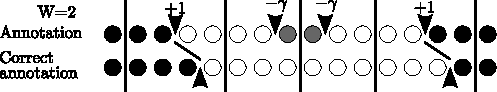
\includegraphics[width=10cm]{../figures/HERDbuddy.pdf}
\end{center}
\caption[Highest Expected Reward Decoding explanation]{
Triangles corresponds to the boundaries. Vertical lines corresponds to the windows
of size $2W$, or smaller to avoid overlaps. Windows around boundaries
represents regions where we search for the corresponding boundaries in the correct
annotation.
The first and the fourth boundary are correctly predicted because in the correct
annotation is boundary between same colors within distance $W=2$.
%correctly predicted (they have penalty $-\gamma$). Because there is no such
%boundary in the correct
%annotation within window.
This picture was taken from \cite{Nanasi2010mgr}.
}\label{FIGURE:HERDBUDDY}
\end{figure}

We say that boundary on position $i$ is correctly predicted, if it satisfy
following conditions.
\begin{enumerate}
\item There is boundary between same labels in the correct annotation on position $j$ and $j$ is
within distance $W$ from $i$ ($|i-j|\leq W$).
\item There is no other boundary between $i$ and $j$. 
\end{enumerate}
Boundaries are illustrated in figure \ref{FIGURE:HERDBUDDY}. 
%In addition, the
%beginning and the end of the sequence are considered to be boundary too (with
%special start and end label).

Let $x$ be the number of correctly
predicted boundaries and $y$ be the number of other boundaries in the proposed
annotation. Then $f(\Lambda,\Lambda')=x-\gamma y$ where $\gamma$ is defined
constant. If $W=1$ then this is equivalent to the Maximum Boundary Accuracy
Decoding. Intuition behind this gain function is that we want to amplify the   
expected gain for the boundary if there are many annotations with similar
boundary.

Optimizing this criteria can be done in $O(|X|W|C||T| + n|C|^2W^2)$ time  and
$O(\sqrt{|X|}|C||V|+W|C||V|+n|C|^2)$ memory. Experimental evaluation,
optimization algorithm and implementation details can be found in
\cite{Nanasi2010,Nanasi2010mgr}.

\subsection{Distance Measures on Annotations}\label{SECTION:DISTANTMEASURES}

Another approach to solve similar problem was proposed by {\it Brown,
Truszkowski} in \cite{Brown2010}. Originally their implementation was aimed at
prediction of boundaries in transmembrane proteins \cite{Brown2010}, but later
they successfully adapted their algorithm to jumping HMMs \cite{Truszkowski2011}.
Their approach is trying to solve same problem as HERD: the exact boundaries of
an annotations are hard to find and grouping similar annotation is useful.
At first we give few definitions.

\begin{definition}
Let $d$ be any distance measure defined on annotations. Ball of radius $r$
around annotation $\Lambda$ is 
\begin{equation*}
B_d(\Lambda,r) = \{\Lambda'\mid d(\Lambda,\Lambda')\leq r\}
\end{equation*}
\end{definition}

\begin{definition}
Let $\Lambda=\Lambda_0\Lambda_1\dots\Lambda_{n-1}$ be an annotations. Footprint
of $\Lambda$ is maximal subsequence of $\Lambda$ that does not contain two
identical 
consecutive labels. \label{DEFINITION::FOOTPRINT}
\end{definition}

\begin{definition}
Let $b_i(\Lambda)$ be $i$-th boundary of $\Lambda$ and $b(\Lambda)$ be the
number of boundaries in $\Lambda$.
Border shift distance $d_{b}$ is 
\begin{equation*}
d_{b}(\Lambda,\Lambda') = \begin{cases}
\infty & \text{if $\Lambda$ and $\Lambda'$ have different footprint}\\
\max_{i=0}^{b(\Lambda)-1} d_i(\Lambda)-d_i(\Lambda') & \text{otherwise}
\end{cases}
\end{equation*}
and border shift sum distance $d_s$ is 
\begin{equation*}
d_{s}(\Lambda,\Lambda') = \begin{cases}
\infty & \text{if $\Lambda$ and $\Lambda'$ have different footprint}\\
\sum_{i=0}^{b(\Lambda)-1} d_i(\Lambda)-d_i(\Lambda') & \text{otherwise}
\end{cases}
\end{equation*}

\end{definition}

To predict the recombinations of sequences or the annotations of the
transmembrane proteins {\it Brown,
Truszkowski} maximize following function
\begin{equation*}
f_d(\Lambda,\Lambda') = 
\begin{cases}
1 & {\text if }\Lambda\in B_d(\Lambda',r)\\
0 & \text{otherwise}
\end{cases}
\end{equation*}

As distance $d$, they have considered Hamming distance, Border shift distance
and Border shift sum distance \cite{Brown2010}.  If we set $r=0$ then $f_d$ is
same as $f_A$ and therefore finding annotation that maximize $f_d$ is NP-hard.

Maximizing $f_d$ is NP-hard but finding the  annotation with footprint $F$ and
maximal expected gain can be done in polynomial time \cite{Brown2010}. Therefore
{\it Brown and Truszkowski} used following heuristic algorithm: At first 
sample the state paths to get the most probable footprint $F$ with high probability,
then use the
polynomial algorithm for finding the annotation with footprint $F$ and the highest expected gain.

Gain function $f_d$ is similar to $f_A$: the annotation is considered correct if
it is same/very similar to the correct one. MBAD, HERD and the
Posterior decoding do not care about overall structure of annotation, they
construct annotation from highly probable features. However,
decoding function $f_d$ take in to account
overall structure of the sequence.




\section{Sequence Alignments}

In this chapter we introduce the sequence alignment problem, basic algorithms
for computing optimal alignments of two sequences as well as several
algorithmic improvements.

Parts of two sequences are homologous, if they have evolved from same sequence
in their common ancestor. Aim of sequence alignment is to identify homologous
sequences. Sequences can be modified by different evolution events:
mutation of a residue into another residue, deletion of a part of the sequence,
insertion of residues into the sequence. There are also large-scale
rearrangement events like duplications (some subsequence is duplicated and
copied into other part of the sequence), inversions (some subsequence is
reversed) or translocations in which part of the sequence change position.  We will
ignore them for now because they cannot be represented by traditional
alignments. An alignment is a data structure that represents comparisons of two
or more sequences. We obtain an alignment of $k$ sequences by inserting dashes
into individual sequences so that they have the same length. We can represent an
alignment as a matrix or a table. Each row of the alignment is a sequence with
inserted dashes, and each column is a list of residues from all rows at the same
position.


An alignment has the following biological meaning: homologous residues (those that
have evolved from a common ancestor) are in same column. Dashes represents
either the parts of sequence that were deleted during evolution (deletions) or
positions where some residues were inserted into some other sequence
(insertions). In an alignment it is not possible to distinguish between insertions and
deletions -- we cannot tell if something was inserted into one sequence or if
there was deletion in the other sequences. Therefore we will refer to insertions
and deletions as to \firstUseOf{indels}.

\begin{example} 
Consider the  following evolutionary history of hypothetical DNA sequences of two
current organisms $X$ and $Y$. There was a parent sequence $P$ which evolved into
$X'$ and $Y'$ and after that $X'$ evolved into $X$ and $Y'$ evolves into $Y$.
These sequences are shown bellow: 
\begin{verbatim}
X:      C C     G C G A C C T T G C             A C C A
X':     C C     G           T T G C             A G C A
P:      A C T G G           T C G C T G A G C T A G C A
Y':     T C T G G           C C           G C T A G C A
Y:      T C T A G           C C           G A T A G C A
\end{verbatim}
%$X$ and $Y$ evolved from parent sequence $P$ through sequences $X'$ and $Y'$.
During evolution from $P$ to $X'$, four events occurred: deletion of 
sequences ``TG''  and ``TGAGCT'' and mutations of two bases. During evolution
from $X'$ to $X$, one base was changed and sequence ``CGACC'' was inserted.  
Similarly during evolution from $P$ to $Y'$, the two bases mutated and two
sequences were deleted. During evolution from $Y'$ to $Y$ one base mutated and
sequence ``CGACC'' was inserted. 

From evolutionary history described above, we can create an alignment of current
sequences $X$ and $Y$ by removing ancestral sequences $X',Y'$ and $P$, 
%\begin{verbatim}
%X:      C C     G C G A C C T T G C             A C C A
%Y:      T C T A G           C C           G A T A G C A
%\end{verbatim}
%We obtain actual alignment by 
removing columns that contain only gaps and
replacing gaps with dashes (gap symbols). 
\begin{verbatim}
X:      C C - - G C G A C C T T G C - - - A C C A
Y:      T C T A G - - - - - C C - - G A T A G C A
\end{verbatim}
In this alignment, symbols that are in the same column are truly homologous (they
evolved from the same symbol in $P$).
%If two residues are in same column in alignment then they are homologous.
As you can see, homologous symbols do not have to be equal.
\end{example}

There is only one alignment that reflects the true evolutionary history. Our goal
is to find this alignment, or at least some alignment, which is as close as
possible. The alignment shown above is a \firstUseOf{global alignment} because it
is an alignment of whole sequences $X$ and $Y$. A \firstUseOf{local alignment}
is an alignment of parts of sequences: a local alignment of sequences $X$ and
$Y$ is a global alignment of strings $\bar{X}$ and $\bar{Y}$ where $\bar{X}$ is
a substring of $X$ and $\bar{Y}$ is a substring of $Y$.  Since global
alignments do not consider rearrangement events\footnote{Duplication, reversal
or translocation.}, local alignments are useful to align sequence parts that
did not underwent such events. We will mostly consider global alignments, but
most of the methods can be extended also to local alignments.

In this chapter we will review basic methods for constructing alignments. We
will discuss basic scoring schemes and algorithms that find optimal alignment
under these schemes. In this thesis we cover mostly probabilistic methods,
which are in section \ref{TODO} and chapter \ref{TODO}.

%At first
%we will discuss pair alignments (alignment of two sequences).
%\correction{Later in this
%chapter we will review some methods how to construct multiple alignments.}{urvat
%ak to nie je pravda}

\subsection{Scoring Schemes}

Since we want to construct alignments that have biological meaning, we have to
develop a method for assessing the quality of an alignment. One way of doing so
is to define a scoring scheme, which assigns to every alignment a real number
(called score). The alignments similar to the true alignment should have higher
score than the alignments that differ from the true alignment. Once we have a
scoring scheme, we will search for the alignment of the input sequences with
the highest score.

Typical scoring schemes used in practice score each column of
an alignment without gaps independently. Gaps are scored by a penalty
that depends on the length of the gap (the number of consecutive dashes). Score
of an entire alignment is the sum of the scores of all ungapped columns plus the
sum of the scores of all gaps.

\todo{Nejake referencie}
In particular
we will assume that all sequences are from a finite alphabet $\Sigma$. For DNA,
$\Sigma=\{A,C,G,T\}$, for proteins $\Sigma$ contains $20$ codes of amino acids.
We will score a column containing residues $a$ and $b$ by $S[a,b]$ where $S$ is
a matrix of size $|\Sigma|\times|\Sigma|$ called \firstUseOf{substitution
matrix}.  A gap of length $x$ has a score $g+dx$, where $g$ is the gap opening
penalty and $d$ is the gap extension penalty. Both are usually negative, since we
want alignments that contains many columns with same or similar symbols. With
positive gap penalty there will be tendency towards alignments with many gaps
which reduce the number of aligned residues.  We call this gap scoring scheme an
affine gap model. 

Matrices and gap penalties used as scoring schemes are usually derived from
frequencies of the substitutions and indels of real alignments. Example of such
matrices are PAM or BLOSUM matrices\cite{Durbin1998}. Additionally, scoring
matrices can be also derived from theoretical models of evolution, one such
example is Jukes-Cantor model\cite{Durbin1998}.

\begin{comment}
Intuition behind this scoring system is probabilistic. Assume that we have
alignment of $X$ and $Y$ without gaps and that each base in DNA evolves
independently. Therefore for every pair of residues $a,b$ there is probability
that $a$ will evolve into $b$. We denote this probability as $p(a,b)$. Therefore the probability that $X$ will evolve
into $Y$ is product of probabilities that $X_i$ will evolve into $Y_i$
\[
\prob{X\text{ evolved into }Y} = \prod_{i=0}^{|X|-1}p(X_i,Y_i)
\]
If $X$ and $Y$ were generated independently be some random model $R$, then probability that we see $X_i$
and $Y_i$ is $\prob{X_i\mid R}\prob{Y_i\mid R}$ ($R$ usually samples symbols
of sequence independently from some distribution). The probability that we $X$
and $Y$ under model $R$ is
\[
\prob{X,Y\mid R} = \prod_{i=0}^{|X|-1}\prob{X_i\mid R}\prob{Y_i\mid R}
\]
As a measure of  $X$ and $Y$ being homologous we take the ratio of the
probability that $X$ evolved into $Y$ and the probability that $X$ and $Y$ are
independent.
By taking logarithm of this ratio we have
\[
\log\left(
\frac{\prob{X\text{ evolved into }Y}}{\prob{X,Y\mid R} }\right)
= \sum_{i=0}^{|X|-1}\log\left(\frac{p(X_i,Y_i)}{\prob{X_i\mid R}\prob{Y_i\mid
R}}
\right)
\]
Therefore by setting $S[a,b]=\frac{p(a,b)}{\prob{a\mid R}\prob{b\mid R}}$ we have one
possible scoring model. $S[a,b]$ is positive if is more likely that $a$ evolved
into $b$ and negative if it is more likely that $a$ and $b$ were generated
independently.  Values of $S$ are usually probabilities multiplied by some
constant and rounded to integers to avoid use of floating point numbers. 

There are two ways of deriving substitution matrices. One way is to derive them
from alignments that were constructed manually by biologists. Such matrices are
for example PAM or BLOSUM matrices. Other possible solution is to use a
theoretical model of evolution, for example Jukes-Cantor model. More details can
be found in \cite{Durbin1998}.
\end{comment}


\subsection{Needleman-Wunsch algorithm}
\label{SECTION:NEEDLE}


The
alignment with the highest score can be found by the Needleman-Wunsch algorithm \cite{Durbin1998}.
This algorithm uses an arbitrary score table $S$, affine gap model with gap penalty
$d$ and gap opening penalty $g=0$ (if $g=0$ then this model is also called
linear gap model). To align sequences $X$ and $Y$ of length $n$ and $m$
respectively, we define matrix $M$ of size $n\times m$. Element $M[i,j]$ will be the
score of the best alignment of sequences $X[:i]$ and $Y[:j]$. We can compute
$M[i,j]$ by the following equations:

\begin{align} 
M[-1,-1] &= 0\\
M[-1,i] &= i\cdot d, 0< i < m\\\
M[i,-1] &= i\cdot d, 0< i < n\\
M[i,j] &= \max
\begin{cases}
 M[i-1,j-1]+S(X_i,X_j)\\M[i,j-1]+d\\
 M[i-1,j]+d
\end{cases}, 0\leq i<n,0\leq j<m \label{ALIGN:ALGO:AFFINE}
\end{align}

By computing $M[n-1,m-1]$, we have the score of the optimal (highest-scoring) alignment of $X$ and $Y$ \cite{Durbin1998}. 

To cope with gap opening penalty, we have to slightly change the algorithm.
We define two other matrices $M_X$ and $M_Y$ of same size as $M$. $M_X[i,j]$
will contain the highest score of an alignment of sequences $X[:i]$ and $Y[:j]$
that ends
with a gap in sequence $X$. $M_Y$ is analogous. Values of these matrices can be computed byy the following recurrences.

\begin{align}
M[-1,-1] &= 0\\
M[-1,i] &= M_X[-1,i] = i\cdot d+g, 0 < i < m\\
M[i,-1] &= M_Y[i,-1] = i\cdot d+g, 0 < i < n\\
M_X[i,-1] &= -\infty, 0\leq i< n\\
M_Y[-1,i] &= -\infty, 0 \leq i< m\\
M[i,j] &= \max
\begin{cases}\label{ALIGN:ALGO:REALAFFINESTART}
 M[i-1,j-1]+S(X_i,X_j)\\
 M_X[i,j]\\
 M_Y[i,j]
\end{cases}, 0\leq i<n,0\leq j<m\\
M_X[i,j] &= \max
\begin{cases}
M[i-1,j]+g+d\\
M_X[i-1,j]+d
\end{cases}, 0\leq i<n,0\leq j<m\\
M_Y[i,j] &= \max
\begin{cases}
M[i,j-1]+g+d\\
M_Y[i,j-1]+d
\end{cases}, 0\leq i<n,0\leq j<m\label{ALIGN:ALGO:REALAFFINEEND}
\end{align}

To compute the
value of $M[i,j]$ (and optionally $M_X$ and $M_Y$), these equations use only values
from neighbouring cells which have at least one coordinate smaller. 
Therefore we can order computation so that when we compute value $M[i,j]$ the
necessary values are already computed.
Let $F$ be
the function, that takes as input matrix $M$  and coordinates $(i,j)$ and computes $M[i,j]$ according equation
\ref{ALIGN:ALGO:AFFINE}.  Let $F'$ be the
same function as $F$, but with $\max$ replaced with $\arg\max$.  Function
$F'(M,(i,j))$ will thus return which cell was used in computation of $F(M,(i,j))$.
Note that if $g$ is not zero, then $F$ would take as input the matrices $M,M_X,$
and $M_Y$ and compute $M[i,j],M_X[i,j],$ and $M_Y[i,j]$ according 
 equations
\ref{ALIGN:ALGO:REALAFFINESTART}-\ref{ALIGN:ALGO:REALAFFINEEND}
%For simplicity, we will assume that both sequences has same length $n$. This
%will allow us to express complexity in simple way.  At first we show how
%to compute compute those algorithms in $O(n^2)$ time and $O(n^2)$

The Needleman-Wunsch algorithm can be implemented by the following code. For simplicity 
we show only computation of matrix $M$.

\lstset{showstringspaces=false}
%\vbox{
\begin{lstlisting}
Initialize M[i,-1] and M[-1,i]
for i in 0...n-1
  for j in 0...m-1
    M[i,j] = F(M,(i,j))
(i,j) = (n-1,m-1)
while i > 0 or j > 0
  (i',j') = F'(M,(i,j))
  (a,b) = (X[i],Y[j])
  if i' = i then a = '-'
  if j' = j then b = '-'
  print column of alignment (a,b)
  (i,j) = (i',j')
\end{lstlisting}
%}

Lines 2-5 fills matrix $M$ and lines 6-12 implement the back-tracing procedure.
Time complexity of this algorithm is $O(mn)$ and memory requirements are $O(mn)$
since we keep matrix $M$ in memory. The algorithm for
affine gap model with $g\not=0$ has the same complexity.


Note that for computing  $i$-th row of matrix $M$ we need only values from row
$i$ and $i-1$. Therefore if we want to know just the score of the optimal
alignment,
we can compute it in $O(m+n)$ memory: after computing of row $i$, we can discard
row $i-1$. However if we want find the optimal alignment, we have to keep matrix
$M$ in the memory or use one of the techniques that are described in section 
\ref{TODO: Aj tak sa to presunie}.

\section{Sequence Alignments with Pair HMM}

\subsection{Pair Hidden Markov Models}\label{SECTION:PAIRHMM}

In this section, we  describe hidden Markov models that generate output on
two tapes, resulting in two emitted sequences. These models are used in
bioinformatics to study relationships between different sequences.

Every state can in one step generate one symbol in each sequence, or one symbol
in one of the sequences or no symbols at all.  Formally, every state generates
a pair of strings $(a,b)$, where $a$ and $b$ are of length at most one.
Moreover, all pairs with generated with nonzero probability by one state have
the same length.  Formal definition of \abbreviation{pair HMMs}{pHMMs} is given
below. We can
use pHMM to define probabilistic scoring schemes for alignments.


In particular, symbols generated by the same state are considered
homologous (are in same column of an alignment). Symbols that are generated by a
state that generates only in one sequence are aligned to a gap. 

\begin{definition}
A \abbreviation{pair hidden Markov model}{pHMM} is a tuple $H=(\Sigma,V,I,d,e,a)$, where $\Sigma$ is a finite
alphabet, $V$ is a finite set of states, $I$ is an initial distribution and $a$ is
a transition matrix, all defined as
in definition \ref{DEF:HMM}. $d^x_v$ and $d^y_v$ are state durations of state $v$
in sequence $x$ and $y$ respectively. For all $v\in V$,
$d^x_v\in \{0,1\}$ and $d^y_v\in \{0,1\}$.
Emission probability matrix $e$ is
a $|V|\times\left(|\Sigma\cup\{\varepsilon\}|\right)^2$ matrix with the following
properties:
\def\lala#1{\{#1\}}
\begin{enumerate}
\item
$\forall v\in V\forall \sigma_1,\sigma_2\in\Sigma\cup\{\varepsilon\}:
0\leq e_{v,(\sigma_1,\sigma_2)}\leq 1$

\item 
$\forall v\in V:
\sum_{\sigma_1,\sigma_2\in\Sigma\cup \lala{\varepsilon }}e_{v,(\sigma_1,\sigma_2)} = 1$

\item For all states $v$ if $e_{(v,\sigma_1,\sigma_2)}>0$ then
$d^x_v=|\sigma_1|$ and $d^y_v=|\sigma_2|$
\end{enumerate}

\end{definition}

A state path is defined the same as for HMMs with silent states. Restriction on
the state durations (condition $3$ in the definition) ensures that given a
state path $\pi$ and emitted sequence $X$ and $Y$, for every symbol from $X$
and $Y$ we can assign a state from $\pi$ that generated that symbol.  However,
given only two sequences $X$ and $Y$ and no state path, it is not possible to
determine which symbols of the two sequences were generated together.

Before we continue, we will define cumulative duration times which will make
further expressions simpler. \todo{koniec feedbacku}

\begin{definition}
Let $\pi=\pi_0\dots\pi_l$ be a state path. Then the \firstUseOf{cumulative duration
times} are
$D^x_i(\pi)=\sum_{j=0}^{i}d^x_{\pi_j}$ and $D^y_i(\pi)=\sum_{j=0}^{i}=d^y_{\pi_j}$.
Additionally, $D^x_{-1}(\pi)=D^y_{-1}(\pi)=0$. If it will be clear from the context
which state path we are using, we will write $D^x_i$ and $D^y_i$ instead of
$D^x_i(\pi)$ and $D^y_i(\pi)$.
\end{definition}

Given sequences $X,Y$ and state path $\pi$ that generated them, we 
can tell which symbols were generated by which states. Since every state $v$
generates exactly $d^x_v$ and $d^y_v$ symbols in $X$ and $Y$ respectively,
state $\pi_i$ generated pair $(X[D^x_{i-1}:D^x_{i}],Y[D^y_{i-1}:D^y_{i}])$
States $\pi_0,\pi_1,\dots\pi_{i-1}$ generated first $D^x_{i-1}$ symbols in $X$
and first $D^y_{i-1}$ symbols in $Y$. 


\begin{example}
In the figure \ref{FIGURE:SIMPLEPHMM} is pair hidden Markov model modeling
sequence alignment with affine gap model. State $M$ is called match state and
generates pair of aligned residues and corresponds to matrix $M$ from the sequence
alignment algorithm. Insert states $I_X$ and $I_Y$ represents gaps,
generates residues in only one sequence and corresponds to matrices $M_X$ and
$M_Y$ from the sequence alignment algorithm from section \ref{SECTION:NEEDLE}.

Note that a state path uniquely define an annotation (match state corresponds to
match columns, insert states represent gap).  Finding the most probable state
path for this HMM is equivalent to the Needleman-Wunsch algorithm with affine gap
model \cite{Durbin1998}.

%\begin{figure}
%\begin{center}
%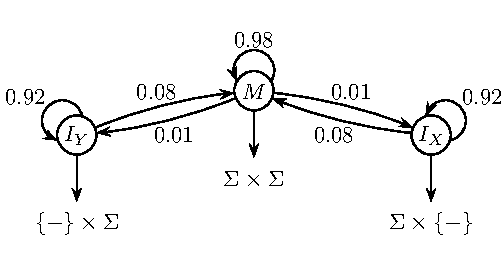
\includegraphics{../figures/simplePairHMM.pdf}
%\end{center}
%\caption[Example of pair hidden Markov model.]{
%State $M$ generates aligned pairs of residues residues, state $I_X$ ($I_Y$) generates
%symbol only in the first (second) sequence.
%}\label{FIGURE:EXAMPLEPAIRHMM}
%\end{figure}
%\section{Use of Pair Hidden Markov Models}\label{SECTION:SIMPLEPHMM}


%We can divide states of pHMM into three types.  Ones that generates symbol in
%both sequences (match states), states that generates symbol in only one sequence
%(indel states) and silent
%states. If pHMM generates  symbols in both sequences we consider those symbols
%to be homologous. We will consider symbols that were not generated by such state
%as indels. Alternative view is to imagine that indel states generate symbol in
%one sequence and gap symbol in the second sequence. In such view pHMM generates
%an alignment.

%Now we show classical pHMM for sequence alignment. It is equivalent to scoring
%scheme of Needleman-Wunsch algorithm with affine gap model. It consists of three
%states: one that generates aligned pairs, and two states for generating
%indels (one for each sequence). Model is shown in figure \ref{FIGURE:SIMPLEPHMM}. 
%
\begin{figure}
\begin{center}
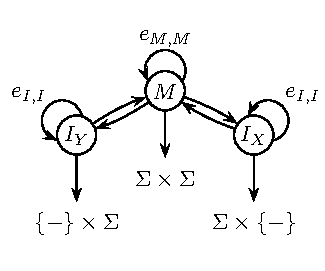
\includegraphics{../figures/pairHMM.pdf}
\end{center}
\caption[Simple pair HMM model for alignment]{Pair hidden Markov model for
pairwise alignment. It has two transitions
parameters $e_{M,M}$ and $e_{I,I}$, since we set $e_{I,M} = 1 - e_{I,I}$ and
$e_{M,I}=\frac12-\frac12e_{M,M}$. Match state $M$ generates aligned pair of symbols
and states $I_X$ and $I_Y$ generates symbols only in $X$ or $Y$ respectively.
Initial distribution is uniform.
}\label{FIGURE:SIMPLEPHMM}
\end{figure}

%As mentioned before, score of the alignment is the probability of state path
%that correspond to such alignment. Therefore we can find the alignment with
%highest score by two dimensional version of Viterbi algorithm. Advantage of
%using this model instead of the Needleman-Wunsch algorithm is that pHMM gives
%probabilistic explanation of the alignments. 



\end{example}

\begin{definition}
Let $H=(\Sigma,V,I,d,e,a)$ be  a pHMM, $X$ and $Y$ be arbitrary sequences over
$\Sigma$ and $\pi$ be a state path. The probability that sequences $X$ and $Y$
were generated by a model $H$  with state path $\pi$ is
\begin{equation}
\Pr\left(X,Y,\pi\mid H\right)=
I_{\pi_0}
\left(
	\prod_{i=1}^{|\pi|}a_{\pi_{i-1},\pi_i}
\right)
\left(
	\prod_{i=0}^{|\pi|}e_{\pi_i,(X[D^x_{i-1}:D^x_{i}],Y[D^y_{i-1}:D^y_{i}])}
\right)
\end{equation}
If $D^x_{|\pi|-1}\not=|X|$ or $D^y_{|\pi|-1}\not=|Y|$ then
$\Pr\left(X,Y,\pi\mid H\right)=0$. 
\end{definition}

Similarly as for HMMs, we can define the probability that sequences $X$ and $Y$ were
generated by the model $H$.

\begin{definition}
Let $H=(\Sigma,V,I,e,a)$ be a pHMM and  $X$ and $Y$ be arbitrary sequences over
$\Sigma$. Then probability that sequences $X$ and $Y$ were generated together by
model $H$ is 
\begin{equation}
\Pr\left(X,Y\mid H\right)=\sum_{\pi}\Pr\left(X,Y,\pi\mid H\right)
\end{equation}
\end{definition}


\subsection{Viterbi algorithm for pair HMM}
\label{SECTION:PAIRHMMVITERBI}
Algorithms operating over pHMMs are similar to those for the regular HMMs, but
in general they have higher computational complexity because they combine
computation  over model states with sequence alignment.  In this section, we
describe two-dimensional version of the Viterbi algorithm, other algorithms are
analogous.

The Viterbi algorithm for HMMs computes variables $V[i,v]$ and $B[i,v]$. Every
variable is parametrized by a position in the sequence and a state. For
two-dimensional version, we will add position in the second sequence.

Let $V[i,j,v]$ be the probability of the most probable state path that generated
$X[:i+1]$ and $Y[:j+1]$ and ended in state $v$. Clearly, $\max_{v\in
V}V[|X|-1,|Y|-1,v]$ is the probability of the most probable state path that
generated $X$ and $Y$. Let $B[i,j,v]$ be the last but one state of the most
probable state path that generated $X[:i+1]$ and $Y[:j+1]$ and ended in state
$v$. To make it easier, we expect that all states but one are not silent -- they emit
symbol in at least one sequence. The one silent state $s$ (start state) will have $I_s=1$.
 Let $n=|X|$ and $m=|Y|$.


\begin{align}
V[-1,-1,s] &= 1\\
V[-2,i,v] &= V[j,-2,v] = 0, \forall v\in V,-1 \leq i < n, -1\leq j < m\\
V[i,j,v] &= \max_{u\in
V}V[i-d^x_{v},j-d^y_v,u]a_{u,v}e_{v,(X[i:i+d^x_v],Y[j:j+d^y_v])}\label{EQUATION:2DVITERBIF}\\
%V[-1,j,v] &= V[i,0,v] = 0 \\
%V[0,0,v] &= I_{v}e_{v,(?,?)} \\
B[i,j,v] &= \arg\max_{u\in
V}V[i-d^x_{v},j-d^y_v,u]a_{u,v}e_{v,(X[i:i+d^x_v],Y[j:j+d^y_v])}\label{EQUATION:2DVITERBIB}
\end{align}

In equations \ref{EQUATION:2DVITERBIF} and \ref{EQUATION:2DVITERBIB} boundaries for $i$ and $j$ are $
-1\leq i< n,-1\leq j< m$ and $i>-1$ or $j>-1$.


By finding the last state $v$ of the most probable state path and back-tracing
from $B[n-1,m-1,v]$ we can reconstruct the most probable state path. Time
complexity of this algorithm is $O(nm|V|^2)$ (or $O(nm(|V|+t)$ where $t$ is the
number of transitions of $H$) and memory requirements are $O(nm|V|)$. However,
we can use various tricks to decrease memory requirements of such algorithms, as
shown in the section \ref{SECTION:ALGORITHMICIMPROVEMENTS}.

\subsection{Generalized Pair HMMs}


A \abbreviation{generalized pair HMM}{GpHMM} (or pair hidden semi-Markov
process) are combination of HMM and GHMM. Every state generates two
duration lengths $d^x$ and $d^y$ from some joint distribution associated with
the current state $d_v(d^x,d^y)$ and after that it generates two strings $x'$
and $y'$ with lengths $d^x$ and $d^y$ according to the joint distribution
$e_{v,(x',y')}$. This probability distribution can by defined for example by
pair hidden Markov model.  As with GHMMs and unlike pHMMs, the state path is not
sufficient to determine which parts of the sequences were generated by which
state, we also need two sequences of durations.

Drawback of GpHMM is increased computational complexity. For example time
complexity of the Viterbi algorithm is $O(nmk^2d^4)$ where $k$
is the number of states of a pHMM and $d$ is the maximum duration length \cite{Meyer2002}.
GpHMMs were successfully used for gene-finding
\cite{SLAM2003,Alexanderson2004,Majoros2005,Meyer2002}. More details are given in
the chapter \ref{CHAPTER:PAIRHMM}.

\subsection{Real life pHMM}
In this chapter we will describe scoring schemes for pairwise sequence alignment
using pHMMs or GpHMM. Scoring schemes used in various programs can differ in the
model they use but also in the decoding algorithm. 
We have discussed the use of pHMMs for sequence alignment in section
\ref{SECTION:PAIRHMM}, where we demonstrated  simple three-state pHMM (figure
\ref{FIGURE:SIMPLEPHMM}) that is equivalent to the
Needleman-Wunsch algorithm \cite{Durbin1998}.  First we 
describe three existing  decoding methods for decoding pHMMs.
The rest of the chapter describes several uses of pHMMs and GpHMM in sequence
alignment or in related problems.

Recall from section \ref{SECTION:PAIRHMM} that a pair HMM generates two
sequences simultaneously and that from state path we are able to recover
annotation.


%In following sections we will review several pHMMs and GpHMMs that were used to
%sequence alignments or other purpose, for example gene finding. We will review
%the application domain of the model, its topology, decoding function, parameter
%estimation and optimisation heuristics. But at first, we have to introduce small
%biological background.

\subsection{Decoding Methods}

In this section we review three decoding methods that were used in literature to
reconstruct pairwise alignments: the Viterbi algorithm, the Posterior
decoding and the Marginalized posterior decoding.

Let $H$ be an pHMM (or GpHMM) and $X$ and $Y$ be the sequences that we want to
align. The probability $\prob{X,Y\mid H}$ is the probability that $X$ and $Y$
were generated in model $H$.  From state path $\pi$ in a pHMM  we can
reconstruct a unique alignment $A_{\pi}$. The model defines the probability 
that
$A_{\pi}$ is the true alignment of $X$ and $Y$ under the assumption, that $X$ and $Y$ were
generated by model $H$:
  \[\prob{\pi\mid
X,Y,H}=\frac{\prob{\pi,X,Y\mid H}}{\prob{X,Y\mid H}}\]
  We can use $\prob{\pi\mid X,Y,H}$ as a score of 
alignment $A_{\pi}$. Path $\pi$ with the highest score can be found by a
two-dimensional version of the Viterbi
algorithm (section \ref{SECTION:PAIRHMMVITERBI}). Alignment $A_{\pi}$ can be
constructed from $X,Y$ and $\pi$ in a straightforward
way: for every match state from $\pi$ that generated $X[i]$ and $Y[j]$ we add
column $(X[i],Y[j])$. For every indel state in $\pi$ that generates $X[i]$ we
add to alignment column $(X[i],'-')$. An indel states for the second sequences are
analogous.  The two-dimensional Viterbi algorithm is used in  most of the
software tools we will discuss later.

Alternatively, we can decode pHMMs using a variant of Posterior decoding.  Two
variants of the Posterior decoding for the pHMMs were described in the
literature: the Posterior decoding and the Marginal posterior decoding
\cite{Lunter2008}.  Let $\prob{X[i]\sim Y[j]\mid X,Y,H}$ be the probability that
$X[i]$ and $Y[i]$ are aligned: the sum of the probabilities of all alignments
that
contain column $(X[i],Y[i])$. Let $\prob{X[i]\sim -_j\mid X,Y,H}$ be the
probability that $X[i]$ is aligned to a gap that is in $Y$ between positions $j$
and $j+1$. Similarly let $\prob{-_i\sim Y[j]\mid X,Y,H}$ be the probability that $Y[j]$
is aligned to a gap in $X$ between positions $i$ and $i+1$. Finally, let
$\prob{X[i]\sim - \mid X,Y,H}$ be the probability that $X[i]$ is aligned to a
gap at any position and let $\prob{-\sim Y[j]\mid X,Y,H}$ be the probability
that $Y[j]$ is aligned to a gap at any position.  Posterior probabilities
defined above can be computed by the two-dimensional version of the
Forward-Backward algorithm (probability that a symbol is aligned to a gap at any position
is the sum of the probabilities that symbol is aligned to a gap at position $i$
for all possible positions $i$).

Let alignment $A$ of sequences $X$ and $Y$ have length $n$ and
consists of columns $a_0,a_1,\dots,$ $a_{n-1}$. Each column is a pair
$a_i=(x_i,y_i)$ where $x_i$ and $y_i$ are symbols from $\Sigma\cup\{-\}$ \footnote{Note that $x$ and $y$ cannot be both gap symbols.}.
Let $d_A^x(i)$ be the number of non-gap symbols in $x_0,x_1,\dots x_{i}$,
let $d_A^y(i)$ be the number of non-gap symbols in $y_0,y_1,\dots, y_{i}$ and
define $d_A^x(-1)=d_A^y(-1)=0$. In this notation, $A[0:i]$ is an alignment of $X[:d_A^x(i)]$ 
and $Y[:d_A^y(i)]$. Then the posterior probability of an alignment column $a_i$ is
\[P(a_i)=
\begin{cases}
\prob{x_i\sim y_i\mid X,Y,H} & \text{if $x_i$ and $y_i$ are not gap symbols}\\
\prob{x_i\sim -_{d_A^y(i)-1}\mid X,Y,H}  & \text{if $y_i$ is gap symbol and $x_i$ not}\\
\prob{-_{d_A^x(i)-1}\sim y_i\mid X,Y,H}  & \text{if $x_i$ is gap symbol and $y_i$ not}
\end{cases}
\]

The \abbreviation{Posterior decoding}{PD} finds the alignment $A$ that maximizes
the product of the posterior probabilities of its columns: 
\[A = \arg\max_{A'\in Al(X,Y)}\prod_{0\leq i <
|A'|}P(a'_i)\] where $Al(X,Y)$ denote the set of all  alignments of sequences
$X$ and $Y$. Similarly we can define \abbreviation{Marginalized posterior
decoding}{MPD}: Let $P'(a_i)$ be the marginalized posterior probability:
\[
P'(a_i) = \begin{cases}
P(a_i) & \text{if $x_i$ and $y_i$ are not gap symbols}\\
\sum_{0\leq j < |Y|}\prob{x_i\sim -_{j}\mid X,Y,H}  & \text{if $y_i$ is gap symbol and $x_i$ not}\\
\sum_{0\leq j < |X|} \prob{-_{j}\sim y_i\mid X,Y,H}  & \text{if $x_i$ is gap symbol and $y_i$ not}
\end{cases}
\]
Then the MPD finds an alignment $A$ that maximizes the product of the
marginalized posterior probability:
\[A = \arg\max_{A\in Al(X,Y)}\prod_{0\leq i < |A'|)}P'(a'_i)\] 

The Posterior decoding and the Marginalized posterior decoding were used by
Lunter {\it et al.} and both produced better alignments than alignments found
by the Viterbi algorithm (more details in section \ref{SECTION:BIASES}). Once
the posterior probabilities of all possible columns of an
alignments are computed (in $O(|X||Y|k^2)$ time where $k$ is the number of
states of pHMM), we can find the alignment that maximizes the desired
function in $O(|X||Y|)$ time. Therefore the time complexity of the PD and MPD is 
$O(|X||Y|k^2)$ \cite{Lunter2008}. 

%Other decoding method can be done by the poster
%Other option is to
%use the  Posterior decoding: for every pairs of residues $X[i],Y[j]$ we compute
%posterior probability that $X[i]$ and $Y[j]$ are aligned $\prob{X[i]\sim Y[j]\mid X,Y,H}$.
%Score of an alignment is sum of posterior probabilities of the aligned residues.
%Later in this chapter we show different variants of the Posterior decoding for
%pHMM.


\subsection{Pair Hidden Markov Models with Gene Structures}

In this section we describe several pair hidden Markov models (or generalized
pair hidden Markov models) with gene structures incorporated into their
topology. These models were used either to align coding DNA or proteins
to a genome or to find genes.


First we introduce several comparative gene finders. Comparative gene finders
use evidence from two organisms to find genes. They use pHMM to simultaneously
align and annotate  two sequences. The advantage finding genes in two
organisms simultaneously is that we can use the evidence from two related
organisms to detect genes that are in both organisms.

\subsubsection{DoubleScan}
Meyer {\it et al. (2002)} developed comparative gene finder DoubleScan.
Generally, DoubleScan has three types of states: {\it match} states, which
generate same number of symbols in both sequences;   {\it emit} states, which
generate sequences only in one sequence and silent states.  

The basic structure of DoubleScan's GpHMM consists of three types of
substructures: substructures that emits exons, substructure that emits introns
and substructure that generate intergenic regions. Each structure has three
copies in the model: one for match states and two for emit states. Exon
substructure is a single state emitting codons (triplets that will be translated
into amino acids).  There is one additional intron substructure connected to
states that generate intergenic regions. This additional intron substructure is
in the model to avoid detecting of pseudogenes. The GpHMM has $54$ states.

%Every such
%structure has three version: one matching version, which emit aligned residues
%and one structure per sequence to emit indels.  Overview of DoubleScan's HMM
%structure is in figure \ref{}. 
\nocite{Meyer2002}

Emission probabilities of the {\it match exon} state were estimated from
relative frequencies in the training set with Dirichlet priors
\cite{Meyer2002,Durbin1998}.  Emission probabilities of other states were
generated  by marginalizing emissions of the match exon state. Transition
probabilities from the initial state were uniform, transition probabilities for
splice sites were estimated by splice site predictor. Other transitions were
observed from training data and tuned by hand.

DoubleScan uses the Viterbi algorithm as a decoding method.  To reduce the
running time of the Viterbi algorithm they use stepping-stone algorithm: first
they run BLASTN to find local alignments. Then DoubleScan chooses a consistent
subset of alignments by the greedy method described in section
\ref{SECTION:SSA}. They restrict the Viterbi algorithm to follow the alignments
in the subset allowing tolerance 15 bases.

\subsubsection{SLAM} 

\begin{figure}
\begin{center}
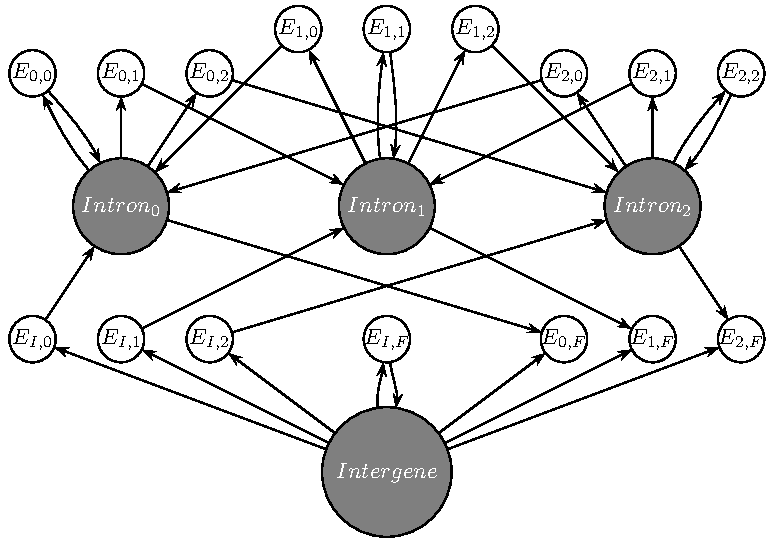
\includegraphics{../figures/slam.pdf}
\end{center}
\caption[HMM topology of SLAM's GpHMM]{
Topology of GpHMM used by SLAM (states for genes on reverse strand are omitted).
Gray states have geometric distribution (modeled with self-loops which are
omitted in the figure). Emissions of shaded states are modeled by the basic
three state pHMM. White states represent exons. Each has associated a duration
distribution and emissions are also modeled by three-state pHMM using $5$-th
order states that emit whole codons at once.  Since introns can be inside a
codon, the model contains an exon state for every possible interruption:
$E_{i,j},0\leq i,j<3$ is an exon that begins with end of the interrupted codon of
length $((3-i)\mod 3)$ and ends with the start of a codon of length $j$. $I$
stands for start codon and $F$ stand for stop codon: states
$E_{I,\cdot},E_{\cdot,F}$ and $E_{I,F}$ model exons adjacent to the beginning
and the end of a gene.  $Intron_i$ models intron that interrupted codon at the
$i$-th position ($0$ means that intron is not interrupting any codon).
}\label{FIGURE:SLAM} \end{figure}

SLAM \cite{SLAM2003}  is a comparative gene finder based on a generalized pair
hidden Markov model \cite{Alexanderson2004} with some states being also
high-order states (with dependence on previous emissions).  It predicts gene
structures for a pair of related eukaryotic organisms. SLAM's decoding method is
the Viterbi algorithm. 

Unlike DoubleScan, SLAM defines a true GpHMM because state durations are not
constant, but are sampled from some distribution (however, distribution they
used is not specified). Topology of the model can be found in figure
\ref{FIGURE:SLAM}.  Emission probabilities of pairs of codons were assigned from
a codon-based PAM matrix.


To reduce the running time of the algorithm first they  align the input
sequences using AVID global alignment tool \cite{Bray2003}. They restrict the
Viterbi algorithm so, that each base matched in the anchor alignment can be
realigned in an interval of size $3$.

\subsubsection{TWAIN}

TWAIN is another approach to use GpHMM to find genes \cite{Majoros2005} and is
interesting because of its decoding algorithm. Twain GpHMM has two types of
states: the states with fixed durations (which emit sequences of fixed length)
and the states with variable duration lengths which are associated with some
distribution.  The states with fixed durations corresponds to specific
signals, such as splice sites, start/stop codons, and so on.
Additionally, the states with variable duration are not connected with each
other; the transitions from/to such states are only to/from states with fixed
duration lengths. Therefore if we know the positions of all signals in the
sequence, we know that sequences between signals were generated by one state.
This can be exploited in the following way.

TWAIN at first annotates input sequences using gene-finder TIGRscan
\cite{Majoros2004} (each sequence is annotated independently) which finds
signals in the sequences and creates a parse graph: vertices of the parse graph are
the signals in the sequence (each signal corresponds to a state of the GpHMM).  Two
signals are connected with an edge if in the genome one signal can follow another:
for example a start codon can be followed by a stop codon or a donor site.
Therefore start codons are connected with following stop codons and
donor sites. Each edge is scored by the probability of the most probable state
path between those two states in the TIGRscan's HMM. To reduce the size of the
graph, some edges are omitted by heuristic.

TWAIN creates graph $G$ by cartesian product of two parse graphs and omits the
vertices that corresponds to pairs of different signals since they are unlikely
to be seen in the alignments. Each node in the graph corresponds to some state $s$
of the GpHMM and cell $c$ in the dynamic programming matrix of the Viterbi
algorithm.   Edges between cells $c_1,c_2$ correspond to alignments
generated by a single state from GpHMM (since states for $c_1$ and $c_2$ are
connected through generalized states).  The Viterbi algorithm is computed only
on cells corresponding to graph $G$ which significantly reduces running time
\cite{Majoros2005}.


\subsubsection{GeneWise}

GeneWise predict genes by aligning a protein  to similar gene structures in DNA
\cite{GeneWise2004}. Instead of pHMM defined as in section \ref{SECTION:PAIRHMM}
it uses probabilistic transducers. Probabilistic transducers are very similar to
pHMM. They are both probabilistic finite state machines, but unlike pHMMs which
generate two sequences, probabilistic transducers transform one sequence into
the other sequence.  The second difference is that transducers have emissions
associated with transitions, not with states.  Therefore transducer emission of
the form $e_{u\to v,(x,y)}=p$ means that during transition $u\to v$ symbol $x$
is read from the input sequence and symbol $y$ is written to the output with
probability $p$ ($x$ or $y$ might also be the gap symbol).  While pHMMs defines
distribution $\prob{X,Y\mid H}$, probabilistic transducers define distribution
$\prob{X\mid Y,H}$, the probability that sequence $Y$ will be transformed to
sequence $X$.

Advantage of transducers over the pHMM is that we can easily compose multiple
transducers together, while maintaining probabilistic interpretation of the
resulting model.  Composition of two transducers $A$ and $B$ is transducer $C$
that transforms sequence $X$ to some sequence $Y$ using transducer $A$ and then
transforms $Y$ to sequence $Z$ using transducer $B$. 

GeneWise model was created by composition of a gene prediction model $S$ which
translates genomic sequence to protein sequence and a protein homology model $T$
which maps protein sequence to a homologous protein sequence.

Gene prediction model $S$ consists of a single exon state which translates
series of codons into amino-acids. It has three submodels for modeling introns,
each consisting of $3$ states representing  splice sites, poly-pyrimidine tract
and central intron section (those $3$ states are associated with $4$
transitions, each transition emit one feature). 

Protein homology model $T$ is a simple pHMM from figure \ref{FIGURE:SIMPLEPHMM}
defined over protein alphabet.  The composition of the models $T$ and $S$ has
$30$ states. Authors removed unnecessary states to reduce the number of states
and transitions \cite{GeneWise2004}.


\subsubsection{Pairagon}

\begin{figure}
\begin{center}
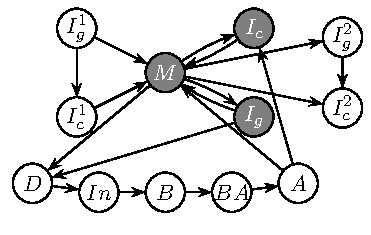
\includegraphics{../figures/pairagon.pdf}
\end{center}
\caption[Topology of Pairagon generalized pair hidden Markov model.]{
Topology of Pairagon GpHMM. All states except states
$D,B$ and $A$ have a self-transition.
Shaded states corresponds to exons: $M$ emits
aligned pairs of symbols, $I_c$ is insertion in the cDNA and $I_g$ is
insertion in the genome. States $I^1_c,I^1_g,I^2_c$ and $I^2_g$ corresponds to
unaligned parts of the DNA and cDNA in the beginning and the end of the
sequences. States $D,In,B,BA,A$ correspond to intron structure and stand for 
Donor, Intron, Branch, Branch Acceptor and Acceptor respectively.
Donor site emits $8$ symbols and acceptor site emits $6$ symbols.
}\label{FIGURE:PAIRAGON}
\end{figure}


The aim of Pairagon is to find local alignments of \abbreviation{complementary
DNA}{cDNA} and genome \cite{Pairagon2009}. By aligning experimentally obtained
cDNA sequences to the genome we are able to confirm intron and exon structures
of genes.  Pairagon's HMM model consists of a simple pair HMM submodel, which
aligns cDNA to DNA and a $5$-state submodel for intron structures. The whole
topology is in figure \ref{FIGURE:PAIRAGON}. 

Model was trained using iterative maximum likelihood approach.  Initial
parameters were trained on the alignments from the \abbreviation{Mammalian Gene
Collection}{MGC}. In this phase, the parameters for intron submodel were set by
hand. The model was then used to align more MGC sequences. Final parameters were
estimated from the new alignments.

Decoding was done by the Viterbi algorithm. Runtime of the algorithm was
improved by the stepping-stone algorithm described in section \ref{SECTION:SSA}
and memory requirements were improved using the Treeterbi algorithm
\cite{Keibler2007}, which is similar to the On-line Viterbi algorithm discussed
in section \ref{SECTION:ONLINEVITERBI}.


\subsection{Non-Geometric Indel Models}
In the simple pHMM described in figure \ref{FIGURE:SIMPLEPHMM}, gap length has
geometric distribution: the probability that a gap has length $n$ is
$e_{M,I}e_{I,I}^{n-1}(1-e_{I,I})$ (note that the probability that at particular
position will be gap with length zero is $1-e_{M,I}$). The Viterbi
algorithm is usually computed in log-space: instead of computing product of
probabilities of events\footnote{Event is emission or transition.}, we compute
the sum of logarithms of those probabilities, because computation in log-space
is numerically more stable. The Viterbi algorithm for the simple HMM
will become the same as the Needleman-Wunsch algorithm.  Gap penalty will be
$\log(e_{M,I})+\log(1-e_{I,I})+(n-1)\log(e_{I,I})$. By setting $d=\log(e_{I,I})$
and $g=\log(e_{M,I})+\log(1-e_{I,I})-d$ we see that this is exactly affine gap
penalty. Therefore we can say that affine gap penalties correspond to geometric
distribution of indel lengths.

As we mentioned in chapter \ref{CHAPTER:ALIGNMENT}, using non-affine gap model
can improve alignment quality.  Problem with geometric distribution (or affine
gap penalties) it that they are not realistic \cite{Cartwright2009,Lunter2008}.
Therefore some other distribution might be more appropriate, for example zeta
distribution \cite{Cartwright2009}, or combination of several geometric
distributions to approximate the distribution of gap length
\cite{Gill2004,Gill2006}.

GpHMM allow us to use arbitrary duration distributions.  On the other hand,
GpHMM are much slower to decode.  One way of incorporating a different gap
distribution into pair hidden Markov models without using their generalized
version is to use several (for example two) indel states for every sequence. For
example Lunter {\it et al. (2008)} used two component mixture models: instead of
one indel state for every sequence they use two. They report that this improved
quality of alignments. Similar approach is used in the multiple sequence aligner
FASTA \cite{Bradley2009}. \nocite{Lunter2008}

Modeling non-geometric distributions with several states can be problematic when
used with the Viterbi decoding \cite{Vinar2005}. Set of states with the same
emission distribution used for modeling non-geometric distribution is called
gadget. We discuss an example of such a problem for the two component mixture
model.

\begin{figure}
\begin{center}
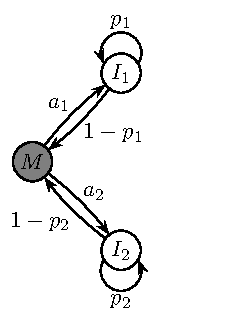
\includegraphics{../figures/twoComponentMixtureModel.pdf}
\end{center}
\caption[The example of an HMM modeling two component geometric distribution]{
Shaded state $M$ represents the match state and states $I_1$ and $I_2$
represents indel states in the same sequence. Indel states for the other
sequence are omitted.
}\label{FIGURE:TWOCOMPONENT}
\end{figure}

Let $H$ be a simple pair hidden Markov model with two pairs of indel states.
Let $I_1$ and $I_2$ be indel states that generate gaps in the first sequence
connected with match state $M$ as in the figure \ref{FIGURE:TWOCOMPONENT}.  Gaps
in alignments (in the first sequence) that are generated by such a model have
length distribution $d(n)=(a_1p_1^{n-1}(1-p_1)+a_2p_2^{n-1}(1-p_2)), n>0$ and
$d(0) = 1-a_1 - a_2$ where $n$ is the length of the gap ($n=0$ means that there
is no gap), $a_1$ and $a_2$ are probabilities of entering state $I_1$ and $I_2$
respectively and $p_1$ and $p_2$ are probabilities of remaining in state $I_1$
and $I_2$ respectively.  This is equivalent to the generalized pair hidden
Markov model $H'$ with one indel state for every sequence which has
$d'(n)=d(n)/(1-d(0))$ as its duration distribution (in generalized states we
want to generate at least one gap. The $d(0)$ should by modeled by the
probabilities of incoming and outgoing transitions to the generalized state). Both models define the same
distribution of alignments  and running the Forward-Backward algorithm or the
Forward algorithm will give the same results. However, alignments constructed by
the Viterbi algorithm can be different for $H$ and $H'$.

Problem is that in the generalized model the Viterbi algorithm gaps of length
$n$ have ``score'' $d(n)$ but in the non-generalized pair hidden Markov model it
will be $m(n)=\max\{a_1p_1^{n-1}(1-p_1),a_2p_2^{n-1}(1-p_2)\}, n>0$ and
$m(0)=1-a_1-a_2$.  These two scores are different ($d(n)$ is always higher) and
therefore it is possible that the Viterbi algorithm reconstruct different
alignments. Therefore if we are using the Viterbi algorithm, we should either
construct a gadget so that $m'(n)$ will be a better approximation of $d(n)$
($d(n)$ is the distribution for the original model) or use a generalized pair
hidden Markov model for the Viterbi algorithm.

%co chcem povedat: niekedy je lepsie pouzit iny gapmodel -- jeden pre kratke
%gapy, jeden pre slhe gapy. Preto sa niekedy 

\subsection{Aligning Sequences with Variable Rate of Evolution}
\label{SECTION:FEAST} 
%\subsection{FEAST} 

The rate of evolution (the expected number of substitution per position in
sequence over some period of time) is not constant for the whole genome. It does
not have to be constant even within one gene. FEAST is pairwise local alignment
tool \cite{FEAST2011} that takes into account the variable evolution rate. The
simple pHMM from figure \ref{FIGURE:SIMPLEPHMM} is optimized for one fixed rate
of evolution.  FEAST contain $k$ such submodels, each trained for a different
rate of evolution.  Submodels are connected with a single silent state.  Since
FEAST is a local alignment tool, it also contains one additional submodel for
generating an unaligned pair of  sequences  at both ends of the sequences.

To construct an alignment (either local or global) FEAST uses the Viterbi
algorithm. Like many local aligners, FEAST uses a seeding heuristics to reduce
computational complexity of finding local alignments.  At first it uses six
different space seeds to get candidate seed and then extends those seeds using
x-drop heuristic \cite{Altschul1997}. The extension is done by an ungapped
version of the Forward algorithm, in contrast with the Viterbi algorithm usually
used for this purpose. 

Estimation of parameters was done by expectation maximization approach (with
Baum-Welsch or Viterbi training). They forced gap parameters to be the same in all
submodels.

Different rates of evolution were also used  in the whole genome aligner GRAPe
\cite{Satija2010}. GRAPe's HMM  consists of two submodels: one with fast
evolution rate and two component geometric mixture model for indels and one with
the lower evolution rate and geometric distribution of indel lengths. GRAPe uses
the Posterior decoding as a decoding method.


\subsection{Biases In Alignments}
\label{SECTION:BIASES}
Lunter {\it et al. (2008)} conducted an extensive survey concerning biases in
alignment. They considered three types of biases associated with gaps. These gap
biases are also discussed in \cite{Durbin1998}. By \firstUseOf{true alignment}
we mean an alignment that corresponds to the actual evolution history.  Since
true alignments are unknown for real data we can simulate evolution on randomly
generated sequences, this obtaining a dataset of ``true'' alignments.

\begin{itemize}

\item \firstUseOf{Gap wander} means that a gap is in a different location that in
the true alignment. Is is due to random short similarities around the borders of
gaps that are indistinguishable from true homologies.

\item \firstUseOf{Gap attraction} is occurs when two gaps are near each other.
In such case merging those gaps and introducing a few mismatches might lead to
higher score. 

\item \firstUseOf{Gap anihilation} occurs when there are two gaps of the same
length, one in each both sequence. Since indels are not so common, removing both
gaps while introducing new mismatches might increase the score of an alignment.

\end{itemize}


Biases are ordered by their frequency from the most occurring to the least
occurring \cite{Lunter2008}. Lunter {\it et al.} explore there problems with a
series of simulations.

They measure the alignment quality by \firstUseOf{sensitivity}, which is the
ratio of the correctly predicted alignment columns to all homologous columns in
the true alignment \cite{Lunter2008}. 

In the first experiment, authors use a simple model of evolution obtaining
alignments with the expected sequence identity $0.705$ with geometric gap model.
The sequences were then realigned using the Viterbi algorithm with the same
model as was used for simulation. Sensitivity was lowest for the  columns near
gaps ($56$\%) and the sequence identity for columns near gaps was $85$\% which
does not agree with the expected sequence identity $0.705$\%.  Moving away from
gaps the average sequence identity dropped to  $0.68$\%. The increased sequence
identity near gaps is due to gap wander bias. The gap attraction effect caused
that the number of gaps that are  near each other was lower than the expected
value obtained from the used gap model.

They also run the Viterbi algorithm parametrized by a range of substitution and
indel rates. The highest sensitivity was obtained for the parameters that were
identical to the parameters used for simulation. However, even then the
sensitivity was only $84$\% indicating that even if we have the right evolution
models, some biases in the alignments are inevitable.  

Lunter {\it et al.} also studied the effect of different decoding methods and
different models on the alignment quality. They simulated evolution with
parameters that are close to the parameters of human-mouse evolution. They
simulated for example the large-scale variation of GC content, GC-content
dependent indel and substitution rates and GC-independent local substitution
rate variation \cite{Lunter2008}.  From simulation they obtained $20,000$
homologous sequence pairs with average length of $700$ nucleotides. They add
flanking sequences of length $100$ nucleotides to the generated sequences  to
simulate local alignments.

After simulation they realigned homologous sequences using the Viterbi algorithm
(VA), the Posterior decoding (PD) and the Marginalized posterior decoding (MPD)
with different models: the three state pHMM ($H_S$); $H_S$ with two indel states
for
every sequence  representing the two component geometric mixture gap model ($H_M$) and the
full model with all parameters that were used for simulation ($H_F$).

They also introduce two additional measures of the alignment quality. The
\firstUseOf{false positive fraction (FPF)} is the proportion of the columns that
are ungapped in the true alignment but wrongly aligned by an algorithm
\cite{Lunter2008}. The \firstUseOf{the nonhomologous fraction (NHF)} is the
proportion of columns containing padding sequence among all columns aligned by
an algorithm.


The use of the different models has little impact on the sensitivity of the
constructed alignments. It is interesting that for the Viterbi algorithm the
sensitivity was lower for the full $H_3$ model than for the simple model $H_1$.
This might be explained by the multiple path problem.  With other decoding
algorithms the models $H_2$ and $H_3$ has slightly higher sensitivity then the
$H_1$ model. 

While the use of the ``better'' model does not significantly improve the quality
of alignments, using the Posterior decoding and Marginalized Posterior decoding
improved the sensitivity by approximately $2.5$\% regardless of the model. On
the other hand the FPF and the NHF was increased with use of the PD and MPD. The
sensitivity of the PD and the MPD were similar but the FPF was lower for the MPD
than for PD. 

The main outcome of this experiment is that proper decoding method can improve
the alignment quality while the use of a simpler model doest not significantly
reduce the alignment quality. However, Lunter {\it et al.} use in their
simulations models only relatively simple models of the evolution. By
incorporating information about gene stricture into alignment models combined
with the use of the right decoding algorithm we can improve alignments further.
This will be discussed in the next chapter. 



\section{Algorithmic improvements}

\section{Algorithmic improvements of sequence alignment}  
%effectively and describe several methods how to decrease memory footprint and/or
%time complexity. 

%As in previous case, values of $M,M_X$ and $M_Y$ can be computed by simple
%dynamic programming and by back-tracing these matrices we can obtain optimal alignment of
%$X$ and $Y$.  Both algorithms have time complexity of $O(nm)$ and memory
%complexity $O(mn)$.  Using tricks described later, the memory and even time
%complexity will be improved.

In this section, we review several techniques that can be used to improve
performance of dynamic programming used to compute sequence alignment.  This is
important, because algorithms described above can be used with sequences that
are several thousands bases long. Full genomes can be several billions bases
long and using naive approach is not tractable. 

\subsection{Restricting Search Space}

One commonly used technique for speedup (and decreasing memory requirements) of
sequence alignment is to restrict the search space of dynamic programming. We
compute alignment only in some parts of matrix $M$ and we assume that omitted
parts of matrix correspond to alignments with low score. 

If the two sequences are quite similar, the optimal global alignment will not be
too far from the main diagonal of matrix $M$. Therefore it is not necessary to compute
parts of matrix $M$ that are too far from the main diagonal \cite{Chao1992} (distance from
diagonal a is
user-defined value or can be computed during alignment \cite{GusfieldBook}).
However, this method is not useful for local alignment or global alignment of 
distant sequences. Now we will discuss some more advanced techniques to
restricting search space of dynamic programming.



\subsubsection{Seeds}

Seeds are a technique frequently  used to reduce time complexity of local
alignment.  They were popularized by BLAST algorithm \cite{Altschul1990}.  A
\firstUseOf{seed} is a short alignment which is likely to be a part of an
alignment with high score. After a seed is found, it is extended with an
extension algorithm to a local alignment.

Seeds that cannot be extended to high-scoring alignments are discarded. Such
candidate seeds are called false positives.  Alignments that were not found by
our heuristics are called false negatives.  It is important that heuristics
used to find seeds has a small number of false negatives and a large number of
true positives, otherwise many true high-scoring local alignments will not be
found. On the other hand, high number of false positives implies longer running
time. 


The most traditional approach is to take as seeds all pairs of positions $i$
and $j$, such that $X[i:i+\tau]=Y[j:j+\tau]$ for some
constant $\tau$. This approach is used in BLAST \cite{Altschul1990}.  Various
generalization were developed to improve trade off between
speed and accuracy, such as seeds with mismatches \cite{Kent2002}, space seeds
\cite{Ma2002}, vector seeds \cite{Brejova2005vector} or daughter seeds
\cite{Csuros2005}.

Extension of a seed to a full alignment is done in both directions, usually
using equation \ref{ALIGN:ALGO:AFFINE} (equation is altered to reverse
direction). Extension is stopped, when some criterion is reached. For example,
BLAST introduced X-drop heuristics: extension stops if the score of an alignment
is lower than the best score that was seen so far minus some user-defined
constant \cite{Altschul1997}.

\subsubsection{Stepping-Stone Algorithm}
\label{SECTION:SSA}

\abbreviation{Stepping-stone algorithm}{SSA} 
\cite{Meyer2002,Pairagon2009} is suitable for global alignment. The idea is to
use good local alignments as anchors. An anchor is similar to a seed: it is a
short alignment which we expect to be in the optimal global alignment.
However, local alignment tools give local alignments that do not have to be
consistent with each other. A set of local alignments is consistent if all
local alignments can be together in one global alignment.
\begin{comment}
Let $A$ and $B$ be a
local alignments of sequences $X$ and $Y$ and $(i,j)$ be the position of the
last alignment column of $A$ in the dynamic programming matrix and $(k,l)$ be
the position of the first alignment column of $B$ in the dynamic programming
matrix. Then $A$ and $B$ are consistent if $i<k$ and $j<l$.  Therefore we need
to choose a consistent subset of alignments.
\end{comment}

SSA chooses a consistent set of local alignments  by a simple greedy method,
always adding highest-scoring alignment consistent with those selected so far.
Selected anchors will be extended to a global alignment. However, since local
alignments may contain errors, SSA will relax them. If $X_i$ and $Y_j$ were
aligned in some anchor, then $X_i$ can be aligned to positions from $j-\tau$ to
$j+\tau$ in the global alignment\footnote{Or aligned to a gap in that region.}
for some user defined constant $\tau$. Similarly, $Y_j$ can be aligned to
positions from $i-\tau$ to $i+\tau$. This technique is also called \firstUseOf{banding},
and it is often used. We used this technique in chapter \ref{TODO}.

\begin{comment}
Time complexity and memory requirements of the stepping-stone algorithm are of
order of $O(\sqrt{|X|^2+|Y|^2})$ under the assumption that the maximum area between
two anchors is independent of the sequence length \cite{Meyer2002}.
\end{comment}

\subsection{Reducing memory complexity}
\begin{comment}
Checkpointing is a general technique in dynamic programming, which allows reduce
the number of rows of the dynamic programming matrix to $O(\sqrt n)$ while
doubling the running time
\cite{Grice1997}. 
\end{comment}
One general technique to reduce the memory requirements of dynamic programing is \firstUseOf{checkpointing} \cite{Grice1997}.

In order to compute the $i$-th row of matrix $M$, we need only row $i-1$. As
mentioned in section \ref{SECTION:NEEDLE}, to compute the score of the best
alignment we need to store only
two consecutive rows.  However, if we want to
recover the optimal alignment, after we have computed its score, we need all
rows of matrix $M$ again, in decreasing order.

Checkpointing solves this problem by storing every $k$-th row of matrix $M$,
$\lceil n/k\rceil$ rows in total.  While back-tracing, we will remember an
additional block $B$ of consecutive $k$ rows in interval $[ik,(i+1)k)$. We can
compute such a block in $O(kn)$ time using the basic dynamic programming,
starting from row number $ik$ which is stored in memory.  Overall, we recompute
every block at most once, and therefore the time complexity will be $O(mn)$.
If we set $k=\sqrt n$ then the memory complexity will be $O(m\sqrt n)$. By
using $l$ recursive applications of this technique we can obtain algorithm with
memory complexity $O(m\sqrt[l]{ n})$.

Even more space reduction can be obtained using the Hirschberg algorithm \cite{Hirschberg1975}. The idea is
the following: if we want an alignment of sequences $X$ and $Y$ that has bases $X_i$
and $Y_j$ aligned, we have to  do dynamic programming only in submatrices
$M_1=M[0:i,0:j]$ and $M_2=M[i:n-1,j:m-1]$. If $i=\lceil n/2\rceil$ then
the total number of cells in those matrices is roughly half of the number of
cells in $M$. The Hirschberg algorithm incorporates a procedure to compute 
$j$ such that $X_i, i=\lceil n/2\rceil$ is aligned to $Y_j$ in optimal alignment of both sequences in $O(nm)$
time and $O(n+m)$ memory. If $X_i$ is aligned to a gap, it finds $j$ such
that $X_i$ is aligned to gap that comes right after $X_j$.
The algorithm then uses such $j$ to determine submatrices $M_1,M_2$ and finds alignments in them recursively.
The optimal alignment is a concatenation of optimal alignments in matrices $M_1$ and
$M_2$.

\begin{comment}
To determine $j$, such that $X_i,i=\lceil n/2\rceil$ is aligned to $Y_j$ (or
$X_i$ is aligned to gap right after $Y_j$) HA uses following algorithm: Let
$B(X,Y)$ be the algorithm, that computes for $X$ and $Y$ vector $LL(k)$, where
$LL(k)=M[n-1,k]$ ($LL$ is the last row of $M$). This can be computed in
$O(nm)$ time and $O(n+m)$ memory using algorithm from section
\ref{SECTION:NEEDLE}.  

We compute a vector $LL_1=B(X[0:i],Y)$. $LL_1[k]$ contains score of the optimal
alignment of $X[0:i]$ and $Y[0,k]$. Let $LL_2[k]$ contains score of the optimal
alignment of $X[i,n]$ and $Y[k,m]$. Then $LL_2=B( (X[i,n])^R,Y^R)^R$.
%which is the last row of the 
%dynamic programming matrix applied to the left part of matrix $M$, and $LL_2=B(
%(X[i,n])^R,Y^R)$, which is the last
%.
%While $LL_1[k]$ contains score of optimal alignment of $X[0:i]$ and $Y[0:k]$,
%$LL_2^R[k]$ contains score of optimal alignment of $X[i,n]$ and $Y[k,m]$.
Searched column $j$ is column that maximizes $\max\{LL_1[j]+d+LL_2[j],
LL_1[j-1]+LL_2[j] \}$.
\end{comment}

Since total size of the two subproblems is always at most half of the size of the
original problem, the running time of the algorithm will be roughly double of
the standard dynamic programming.
The Hirschberg algorithm keeps in memory only a constant number
of rows of $M$,  and therefore the memory requirements are
$O(n+m)$. The Hirschberg algorithm reduces memory more than checkpointing, 
However, checkpointing can be applied to a wider class of algorithms, as we will
see in section \ref{SECTION:HMMCHECKPOINTING}.

\subsection{Exploiting Sequence Repetition}

This technique reduce time complexity of alignment algorithm to $O(n^2/\log n)$
This idea combines LZ78 factorization \cite{Lempel1976} and
$O(A+B)$ algorithm for computing row minima/maxima in totally a monotone matrix of
size $A\times B$ \cite{Aggarwal1987}. We will discuss only two main ideas behind
this algorithm. 
%This technique is the extension of the four-russian trick to
%unrestricted cost matrices. Four-russian trick use clever precomputation to
%speed up sequence alignment \cite{GusfieldBook}

\subsubsection{Totally Monotone Matrices}
\todo{Vyrazne skratit + spomenut 4 rusov ako originalnu techniku. + este by sa oplatilo spomenut tie rozne gap funkcie, aspon citacie na ne by to bolo treba}

\begin{definition}\cite{Crochemore2002}
A Matrix $M$ of size $n\times m$ is \firstUseOf{totally monotone} (with concave condition),
if and only if for all $0\leq i,j< n, 0\leq k<l<m$ the following condition holds:
if $M[i,k]\leq M[j,k]$ then $M[i,l]\leq M[j,l]$.
\end{definition}

If $M$ is totally monotone, then we can compute maximum of every row 
in $O(n+m)$ time by SMAWK algorithm \cite{Aggarwal1987} (This problem is called
\firstUseOf{row maxima}).

\begin{definition}\cite{Crochemore2002}
Let $M$ be a matrix and $M'$ be its
submatrix. \firstUseOf{Input border} $I_{M'}$ of $M'$ is the left column and top
row of $M'$ and \firstUseOf{output border} $O_{M'}$ of $M'$ is the right column and
bottom row of $M'$. Elements of $I_{M'}$ are ordered in clockwise direction
and elements of $O_{M'}$ are ordered in counter-clockwise direction.
\end{definition}

Intuition behind input and output border is following. If we look on the
computation of alignment algorithm inside submatrix $M'$, input border is input
to this computation and output border is output of this computation.

\begin{definition}\cite{Crochemore2002}
Let $M'$ be submatrix of $M$, $I_{M'}=\{i_0,i_1,\dots,i_{k-1}\}$ be its input
border, and $O_{M'}=\{o_0,o_1,\dots,o_{l-1}\}$ be its output border. Then
matrices
$DIST$ and $OUT$ of size $k\times l$ are defined in following way:
$DIST[a,b]$ is the cost of optimal alignment from cell $i_a$ to cell $o_b$.
$OUT[a,b]=i_a+DIST[a,b]$.
\end{definition}

Clearly, $o_b=\max_{0\leq a < k}OUT[a,b]$. Therefore by computing row maxima in
matrix $OUT$, we can compute values of output borders. Matrices $DIST$ and $OUT$
are totally monotone \cite{Crochemore2002}.  If we have matrices $DIST$ and
$OUT$ in advance and $M'$ is of size $m'\times n'$ then we can compute values of
output border in time $O(n'+m')$ by the SMAWK algorithm.

Now we show how to divide matrix $M$ into several submatrices so that
it is possible to efficiently represent matrices $DIST$ and $OUT$.

%Let $M$ be dynamic programming matrix for alignment algorithm for some sequences
%$X$ and $Y$. Let $M' =
%M[i:j,k:l]$ be rectangular submatrix of $M$. Values of $M'$ depends on 
%values cells in submatrices $M[i-1,j:l]$ and $M[i:k,j-1]$ and on value
%$M[i-1,j-1]$. Let $I_{M'}$ be the set of such cells. Let $O_{M'}$ be the 
%the set of cells in $M[i-1,j:l]$ and $M[i:k,j-1]$ (the cells in the top row or
%right column of $M'$). Let $I_0,I_1,\dots$ be enumeration of cells in $I_{M'}$
%and $O_0,O_1,\dots$ be enumeration of cells in $O_{M'}$.  Now we will construct
%the  matrix $DIST_{M'}$ of size $|I_{M'}|\times|O_{M'}|$ where  
%$DIST_{M'}[i,j]$ is the cost of optimal alignment from cell $I_i$ to cell $O_j$.
%Let $OUT[i,j]=I_i+DIST[i,j]$. Both $DITS$ and $OUT$ are totally monotone with
%convex condition 


\subsubsection{LZ78 factorization}

LZ78 is a compression algorithm that uses a dynamic dictionary, which is being built
while the sequence is compressed \cite{Lempel1976}. The way how it parses the sequence
can be used to accelerate dynamic programming \cite{Crochemore2002,Weimann2009}. 
LZ78 factorization divides
sequence $S$ into $k$ strings $S_0,\dots,S_{k-1}$, where $S_0S_2\dots S_{k-1}=S$ and
for every index  $i,0< i <k$ there is index $0\leq j<i$ such that $S_j$ is
prefix of $S_i$ of size $|S_i|-1$. We will call $S_j$ to be a
\firstUseOf{predecessor} of $S_i$.  We have guarantee that the number of strings
$k$ is in  $O(\frac{n}{\log n})$ where $n$ is the length of $S$
\cite{Lempel1976}. 

To align sequences $X$ and $Y$, we factorize them into sequences of strings
$\{X_i\}_{0\leq i < k_x}$ and $\{Y_i\}_{0\leq i<k_y}$.  Every pair $(X_i,Y_j)$
defines a rectangular submatrix $B_{i,j}$ of $M$.  All $B_{i,j}$ are
disjoint and all blocks cover matrix $M$. We say that block $B_{k,l}$ is
a predecessor of block $B_{i,j}$ if one of the following conditions is true:

%If we want to align sequences $S$ and $T$, we factorize $S$ and $T$
%into sequences of strings $\{S_i\}_{0\leq i < k_s}$ and $\{T_i\}_{0\leq i<
%k_t}$. Every pair $(S_i,T_j)$ defines rectangular block of matrix $M$.
%We say that $(S_k,T_l)$ is predecessor of $(S_i,T_j)$ if one of the following
%conditions is true:

\begin{itemize}
\item $X_k$ is predecessor of $X_i$ and $l=j$
\item $k=i$ and $Y_l$ is predecessor of $Y_j$
\item $X_k$ is predecessor of $X_i$ and $Y_l$ is predecessor of $Y_j$
\end{itemize}

Note that every block has $0,1$ or $3$ predecessors. Only block
$B_{0,0}$ has $0$ predecessors and only blocks $B_{i,0}$ and $B_{0,i}$
($i>0$) have only $1$ predecessor.  

%\todo{Mozno by nebolo odveci popisat aj tu strukturu, ak bude cas} NEBUDE
{\it Crochemore et al.} described a data structure that represents $DIST$ and $OUT$
matrices for  \nocite{Crochemore2002} individual blocks $B_{i,j}$. Structures
for $B_{i,j}$ can be
computed from $DISTS$ and $OUT$ matrices of theirs predecessors in time
$O(|X_i|+|Y_j|)$. Details of this algorithm can be found in
\cite{Crochemore2002}. Time complexity of this algorithm is proportional to the
sum of the sizes of all blocks, which is $O(n^2/\log n)$ where $n$ is the length
of the longer sequence.




\begin{comment}
\section{Non-Affine Gap Models} 


%\todo{Mozno by sa dalo dodat aj viac citacii} 
The reasons why affine gap models are
used in sequence alignment are that they are simple, easy to compute and give
reasonable results. While affine gap scoring works fine for short gaps, penalty
for long gaps is too high. Use of different gap models can improve quality of
reconstructed alignments \cite{Gill2004,Cartwright2009}.

Let $f(x)$ be the gap penalty for a gaps of length $X$.
In 
affine gap models, this function has the form $f(x)=g+dx$. For general gap function, we have to
reformulate equation \ref{ALIGN:ALGO:AFFINE} for computing the highest scoring
alignment in following way:
\begin{align}
M[i,j] &= \max
\begin{cases}
 M[i-1,j-1]+S(X_i,X_j)\\
 \max_{x\leq j}M[i,j-x]+f(x)\\
 \max_{x\leq i}M[i-x,j]+f(x)
\end{cases}, 0<x\leq i<n\label{ALIGN:ARBITRARYGAPEQUATION}
\end{align}
This algorithm has time complexity of $O(n^3)$, where $n$ is the length of the
longer sequence. Note that this was the original Needleman-Wunsch 
algorithm \cite{Needleman1970}, and later it was improved to $O(n^2)$ algorithm
\cite{Sankoff1972} for alignment with linear gap penalties.
Unlike previous recursive equations, in this algorithm $M[i,j]$ depends not
only on neighbouring cells, but also on all previous cells in the same row and column.
Therefore some memory-saving techniques like Hirschberg algorithm or checkpointing cannot be
used with general gap penalties.


\subsection{Convex/Concave Gap Functions}\label{SECTION:CONVEX}

Arbitrary gap penalties increased running time of the Needleman-Wunsch algorithm
by factor of $O(n)$. However if we place some
restrictions on the  gap penalty function, we can use faster algorithms. In this
section, we
show an algorithm that computes the optimal alignment in $O(nm\log n)$ time if
the gap
penalty is convex or concave. In some cases this algorithm can be improved to
$O(nm)$ time. This algorithm was discovered independently by Miller
{\it et al. (1988)} and Galil {\it et al. (1989)} \nocite{Miller1988,Galil1989}.

We will present a variant of $O(nm\log n)$ algorithm for convex gap functions which
we believe is easiest to explain . Algorithm for concave gap function is similar.
We consider only convex functions defined on natural numbers (gap length can be only
natural number). Our definition of convex function is similar to one used in
\cite{GusfieldBook}.


\begin{definition}
We assume that $f(x)$ is a  function defined on natural numbers. Function $f$
is convex if and only if 
\[f(x+1)-f(x)\geq f(x)-f(x-1)\]
for all $x\in\mathbb{N}$.
\end{definition}
\begin{note}
It is easy to show that if $f$ is convex then $f(x+d)-f(x) \leq f(x+e+d) -
f(x+e)$ for nonnegative $d$ and $e$.
\end{note}

We will improve dynamic programming that computes matrix $M$ using equation
\ref{ALIGN:ARBITRARYGAPEQUATION}. The increase in running time is caused by two
terms: $M[i,j-y]+f(y)$ and
$M[i-x,j]+f(x)$. In dynamic programming from section \ref{SECTION:NEEDLE} we  have
to add additional nested cycles that go through all values $x$ and $y$. We show
a data
structure that can compute $\max_{0\leq y < j}M[i,j-y]+f(y)$ in $O(\log n)$
amortized time.
This data structure can also handle the second problematic term, but we
will describe only the first one. First we change the variable in the
maximization so that we maximize

%$\max_{0\leq y < j}M[i,j-y]+f(y)$ is equivalent to
\begin{equation}
\max_{0\leq k < j}M[i,k]+f(j-k)\label{CONVEX:MAXFUNCTION}
\end{equation}
which is equivalent to the original expression from the equation
\ref{ALIGN:ARBITRARYGAPEQUATION}.  Our data structure is a list $L_j$ containing
values of 
$k$ that can become maximum for future values of $j$. We will try to keep this list as small as
possible. List $L_j$ will be a called \firstUseOf{candidate list} and members of $L_j$
will be called \firstUseOf{candidates}. Rank of candidate $k$ is the value
$G(k,j)=M[i,k]+f(j-k)$. To compute $M[i,j]$ we iterate over values of $k$ in
$L_j$ and find the one with the highest rank.
%$L_j$ is candidate list for computing $M[i,j]$. 
List $L_{j+1}$ will be computed from $L_j$ by adding $j$ and
removing some elements of $L_j$. 
%For simplicity, let $G(k,j) = M[i,k]+f(j-k)$.
%If $k\in L_j$, than \firstUseOf{rank} of $k$ is $G(k,j)$. 
Note that the rank of
candidates will change when we move from $L_j$ to $L_{j+1}$.

We will explain this algorithm in iterative way: we will be adding to algorithm
new features until it will have desired time complexity. 

%Let $L_j$ be the list of such $k$'s. We will call $L_j$ a \firstUseOf{candidate
%list} and members of $L_j$ \firstUseOf{candidates}. $L_j$ will be created from
%$L_{j-1}\cup\{j-1\}$ by removing some elements. Let $G(k,j) =
%M[i,k]+f(j-k)$.  \firstUseOf{Rank} of candidate $k$ is $G(k,j)$.  i
The trivial algorithm includes all values smaller than $j$ in $L_j$.
%We start with $L_j$ containing all $k$ that are smaller then $j$.  We can find
%element with maximal rank by computing rank for all candidates from candidate
%list $L_j$. 
This leads to $O(j)$ time for finding maximum and $O(1)$ for update
from $L_i$ to $L_{i+1}$
%candidate list (we have to add element $j$ to list $L_{j}$ to create
%list $L_{j+1}$). 
This is equivalent to the original Needleman-Wunsch algorithm
\cite{Needleman1970}. 
We will use the following lemma to
decrease size of candidate lists. This lemma and proof is  slightly modified
from 
\cite{GusfieldBook}.


\begin{lemma}\label{OneStrikeAndOut}
If $G(k,j)\leq G(k',j)$ for some $k<k'<j$, then
$G(k,j')\leq G(k',j')$ for all $j'\geq j$. 
\end{lemma}


\begin{proof}

Inequality $M[i,k]+f(j-k)\leq M[i,k']+f(j-k')$ implies that
$M[i,k]-M[i,k']\leq f(j-k')-f(j-k)$. From convexity of $f$ we have
$f(j-k')-f(j-k)\leq f(j'-k')-f(j'-k)$, and therefore
$M[i,k]-M[i,k']\geq f(j'-k')-f(j'-k)$ which 
is equivalent to
$M[i,k]+f(j'-k)\leq M[i,k']+f[(j'-k')$ or $G(k,j')\leq G(k',j')$.

\end{proof}

Using this lemma, we can improve our algorithm.
Once we find out that $G(k,j)\leq
G(k',j)$, for $k<k'$, we can remove $k$ from $L_{j'}, j'\geq j$ without
affecting the result
of the algorithm, because rank of $k$ will remain smaller than rank of $k'$ for
all $j'\geq j$.
When we move from $j$ to $j+1$, we therefore set $L_{j+1}=L_{j}\cup\{j\}$ and
then
we remove from $L_{j+1}$ that candidates that have lower or equal rank than the 
candidate following them in the list.
%when we move from
%$j-1$ to $j$ we add set $L_j=L_{j-1}\cup\{j-1\}$ and we compute $G(k,j)$ for
%all $k\in L_j$ and remove all such $k$ where there exists $k'\in L_j$ such that
%$G(k',j)\geq G(k,j)$. i
This can be done in $O(|L_{j}|)$ time. Candidates in the resulting list,
$L_{j+1}$ will have decreasing rank. Therefore the first item in
$L_{j+1}$ is the maximal one, so we can find it $O(1)$ time.  This change
does not improve the worst-case behaviour of our algorithm, but it might
significantly reduce the  size of $L_j$ in practice. 


Using this algorithm, $L_j$ will be always ordered by rank. However when we move
from $j$ to $j+1$, the ranks will change, and we have to remove some elements 
to restore this property. The algorithm can be improved if we can compute the column in
which two adjacent  candidates will brake the ordering.

%Nice property of $L_j$ is that it's members are ordered by rank. However, 
%when we move to column $j+1$, ranks of candidates will change and order might be
%broken and therefore we have to traverse through whole $L$ to fix that.
\begin{definition}
For $k<k'$, let $H(k,k')=l$ be the minimal $l$ such that $G(k,l)\leq G(k',l)$. If such $l$ does
not exists,  $H(k,k')=\infty$ 
\end{definition}

If the rank of $k$ is greater than the rank of $k'$ then $H(k,k')$ is the first
column $j'$
 where the rank of $k$ is less than or equal to the
rank of $k'$. Candidate $k$ will be removed in column $j'$, or possibly earlier.  Note that
such $l$ can be found using binary search (based on lemma \ref{OneStrikeAndOut})
in $O(\log n)$ time for any convex function. For some convex functions we can
find it analytically in constant time.


We can further decrease the size of the candidate list using the following
lemma.

\begin{lemma}\label{TimeLemma}
Let $k,k',k''\in L_j$ and $k<k'<k''$. If $H(k,k')\geq H(k',k'')$, element $k'$ can be
removed from $L_j$.
\end{lemma}

\begin{proof}
Since candidates in $L_j$ are ordered by rank, $G(k,j)>G(k',j)>G(k'',j)$.
From definition of $H$ we know that 
$G(k',j')\leq G(k'',k')$ for  all $j'\geq H(k',k'')$. Since
$H(k,k')\geq H(k',k'')$, then $G(k,j')\geq G(k',j')$ for all $j'<H(k,k'')$.
Therefore the rank
of $k'$ will never be maximum and $k'$ can be removed.

%and both are in $L_j$ then $k$ has higher rank that $k'$. Therefore
%it is not maximum. $k'$ have in $H(k',k'')$ lower rank and will be removed from
%candidate list (using lemma \ref{OneStrikeAndOut}). However, since $H(k,k')\geq
%H(k',k'')$ rank of $k'$ will never be maximum.
\end{proof}

Now we can formulate the final algorithm. After updating $L_j$ from $L_{j-1}$,
$L_j$ will satisfy the following invariant.
\begin{invariant}\label{LogGapInvariant}
All consecutive elements $k,k'$ in $L_j$ satisfy the following properties:
\begin{enumerate}
\item $k<k'$
\item $G(k,j)>G(k',j)$ (decreasing rank)
\item if $k'$ is not the last element of $L_j$ and $k''$ is the element
following $k'$
in $L$, then $H(k,k')> H(k',k'')$ (increasing ``time'' when consecutive
candidates will brake the ordering of ranks)
\end{enumerate}
\end{invariant}

Since the rank is decreasing, we can find the maximum in $O(1)$ time. Now we show how
to compute $L_{j+1}$ from $L_j$. Let $L$ be our working list,
$L[k]$ be its $k$-th element, and $l$ be the index of the last element of $L$. 
List $L_{j+1}$ can be computed by the following algorithm. 
\begin{enumerate}
\item $L=L_j$
\item $L_{j+1}=L\cup\{j\}$.
\item If $G(L[0],j+1)\leq G(L[1],j+1)$ then remove $L[0]$ from
list (lemma \ref{OneStrikeAndOut}).
\item While $H(L[{l-1}],L[{l}])\leq H(L[l-1],L[l-2])$ or $G(L[l],j+1)\geq
G([l-1],j+1)$, remove $L[l-1]$ from the list (lemma
\ref{TimeLemma} and lemma \ref{OneStrikeAndOut}).
\end{enumerate}

The first element is also the first element that can break order, so we have to
test it (step 3). Since we add candidate $j$, we have to remove from the end of
the list all candidates with smaller rank than $j$ and those that can be removed
based on lemma \ref{TimeLemma} and lemma \ref{OneStrikeAndOut}.  Since both
ranks and times are ordered, we need to remove candidates only from the end of
the list.

It is easy to see that if $L_j$ satisfies the invariant, $L_{j+1}$  satisfy it.
It is also clear that this algorithm will never remove any candidate that will
be the maximum later, which implies the correctness of the algorithm.

The algorithm described above has running time $O(l\log(n))$, but the amortized time
complexity for computing all columns of one row of matrix $M$ is $O(n\log n)$ since every candidate will
be added/removed to/from list at most once. If we can compute function $H$ in
constant time, the time complexity is $O(n)$.

Using this algorithm, we can compute the optimal alignment with convex gap functions in
$O(nm\log n)$ time and in $O(nm)$ time  if $H$ can be computed
in constant time.

There is also a more complicated $O(nm\alpha(n))$ algorithm for this problem
\cite{Klawe1990}, where $\alpha(n)$ is the inverse Ackermann function. This algorithm
is very complex, and we doubt that it is useful in practice. However, we are
not aware of any experimental comparison of these two algorithms.




%tu chcem definiciu convexnej gap funkcie
%algoritmus ktory je v case n^2 log(n)
%algoritmus, ktory bezi v case n^2 alpha(n)
%kubicky algoritmus v worstcase, ale prakticky konstantny (budem musiet najst 
%citaciu -- nepodarilo sa mi to najst. Zaujimave\ldots)

\end{comment}

\section{Algorithmic Improvements For HMMs}
\label{SECTION:ALGORITHMICIMPROVEMENTS}

In this section we review implementation details and several algorithmic
improvements of the Viterbi algorithm and the Posterior decoding for HMMs and
pHMMs. Mostly we will assume that HMMs does not have silent states.  Most of these
techniques are easily adjustable to HMMs with silent states. 

\subsection{Basic Implementations}

Implementation of the Viterbi algorithm and the Forward-Backward algorithm can be
done by a two-dimensional dynamic programming, similarly as with the sequence
alignment. Let $H$ be an HMM, $V[i,v]$ be  $n\times m$ matrix where $n$ is the
length of the sequence and $m$ is the number of states of the HMM. $V$ will be the
dynamic programming matrix for the Viterbi algorithm or the Forward algorithm.

Code for the Viterbi algorithm is following:
\begin{lstlisting}
Initialize D[0,*]
for i = 1...n-1:
  for v = 0...m-1:
    V[i,v] = max    [u=0...m-1] V[i-1,u]*[v,X[i]]*a[u,v]
    B[i,v] = argmax [u=0...m-1] V[i-1,u]*[v,X[i]]*a[u,v]
statePath[n-1] = argmax [u=0...m-1] V[n-1,u]
for i=n-1...1:
    statePath[i-1] = B[i,statePath[i]]
\end{lstlisting}

This algorithm runs in $O(nm^2)$ and requires $O(nm)$ memory. Note that values
of row $V[i,\cdot]$ and $B[i,\cdot]$ are computed from rows $V[i-1,\cdot]$ so if
we want just the probability of the most probable state path, we need to
remember only last two rows of $V$ (and we do not need $B$) so the memory
requirements will be $O(n+m)$. If we replace on line $4$ maximum with summation
and remove lines $5-8$, we will obtain the Forward algorithm. Lines $6-8$
implements back-tracing procedure, which will be omitted in the Forward
algorithm. The Backward algorithm is analogous to the Forward algorithm.

Note that if $a[u,v]$ is zero, then value on the right side of lines $4$ nd $5$
is zero. Therefore we have to iterate only for such $u$, that $u\to v$ is
transition in $H$. By this we will reduce time complexity to $O(n(m+t))$ where
$t$ is the number of transitions of $H$ not only for the Viterbi algorithm, but
also for the Forward algorithm and the Posterior decoding.


\subsection{Checkpointing}
\label{SECTION:HMMCHECKPOINTING}
Checkpointing can be used to decrease the memory complexity of the Viterbi
algorithm with back-tracing procedure and the Posterior decoding to $O(\sqrt n
m)$.  Similarly, this technique can be used to reduce memory complexity of the
algorithms for pHMMs to $O(nm\sqrt n )$ where $n$ is the length of the longer
sequences and $m$ is the number of states of HMM.

\subsubsection{The Viterbi Algorithm}
While back-tracing, we need access to values of matrix $B$ in decreasing order.
We need only matrix $B$ and last row of $F$. From $i$-th row of $F$ we can
recompute $i+1$-th row of $B$. Therefore we will remember every $k$-th row
of $V$ from which we will recompute blocks of matrix $B$. $B$ will be split into
blocks
$B_0=B[1:k+1,:],B_1=[k+1:2k+2,:],\dots,B_i=B[ik+1:{i+1}k+1,:],\dots$
We will keep in the memory exactly one block of $B$. If we need row that is in block
$B_i$ but $B_i$ is not in memory, we discard current block and compute block
$B_i$ from $V[ik,\cdot]$. Since we need rows of $B$ in decreasing order, we
recompute every block exactly once. If $k=\theta(\sqrt n)$ then the memory
complexity is  $O(n+m\sqrt n)$.

For two dimensional version we keep every $k$-th matrix $V[ik,\cdot,\cdot]$.
Algorithm is analogous to one-dimensional version or to the checkpointing
technique for the Needleman-Wunsch algorithm

\subsubsection{The Posterior Decoding}

In the Posterior decoding need to interlace computations of $F[i,v]$ and
$B[i,v]$ to compute $F[i,v]\cdot B[i,v]$ for all $0\leq i<n,v\in V$. We will
compute $F$ using the checkpointing technique (we compute every $k$-th row of
$F$ and keep in memory only one block).  $B[i,v]$ will be computed row by row
with the version of the  Backward algorithm that need only $O(m)$ memory. When
we compute $B[i,v]$, we also compute $F[i,v]$ by checkpointing technique (if $i$ is in
current block then return $F[i,v]$ from current block. Otherwise discard current
block and recompute the block for row $i$). With this approach we can
compute the posterior values with the $O(m\sqrt n)$ memory. We recompute every row at most
once and therefore the time complexity is $O(n(m+t))$.

\begin{comment}
\subsection{Using Sequence Repetition}

This techniques uses dictionary based encoding schemes to speedup calculation of
algorithms. We will show how to use this technique to Forward algorithm. Details
about how to use this technique to other algorithms can be found in
\cite{Lifshits2009}.


Idea of this speedup is that we reformulate Forward algorithm into sequence of
matrix multiplications.
Let $H=(\Sigma,V,I,e,a)$ be a HMM, $|V|=m$.  Let $M_x[u,v]=a_{u,v}e_{v,x},
u,v\in V,x\in \Sigma$ be the $m\times m$ matrix and $I_x[u]=I_ue_{u,x}$ be
$1\times m$ vector. Matrix $M_x[u,v]$ corresponds to the transition from the
state $u$ to the state $v$ with emission of $x$ from the state $v$.

\begin{lemma}\label{LEMA:MATRIXMULTI}
Let $X=X_1\dots X_n$ be a sequence, $H$ be a HMM and $M_x$ and $I_x$ defined as above and
$F[i,\cdot]$ be row vector from the Forward algorithm.
Then
\begin{align}
F[0,\cdot] &= I_{X_0}\\
F[i,\cdot] &= I_{X_0}\prod_{j=1}^i M_{X_j}
\end{align}
for all $i< n$.
\end{lemma}

\begin{proof}
We prove this lemma by induction.  If $|X|=1$ then
$F[0,v]=I_{X_0}[v]=I_{v}e_{v,X_0}$ for all $v\in V$.  Assume that for
$F[k,:] = I_{X_0}\prod_{j=1}^k M_{X_j}$ (note that the  product of zero matrices
is the identity matrix). We have 
\begin{align*}
\left(I_{X_0}\prod_{j=1}^{k+1} M_{X_j}\right)[v] &= 
\left(F[k,:] M_{X_{k+1}}\right)[v]\\ &= \sum_{u\in V} F[k,u]
M_{X_{k+1}}[u,v]\\ &= \sum_{u\in V} F[k,u] a_{u,v}e_{v,X_{k+1} } \\&= F[k+1,v] 
\end{align*}
for all $v$. 
\end{proof}

Consequence is that we can write the Forward algorithm as the sequence of
multiplications of $|\Sigma|$ different matrices. Since matrix multiplication
is associative, we can use repetitive patters to speedup the calculation. 
Let $x$ be a subsequence of $X$ that has $k>1$ non-overlapping occurrences in $X$.
We can compute $M_{x[0]}M_{x[1]}\dots M_{x[{|x|-1}]}$ once and use it several
times. Let $M_{x}=\prod_{i=0}^{|x|-1}M_{x[i]}$ for any string $x$.

By proper choosing of substrings $x$ we can speedup computation of the Viterbi
algorithm\footnote{For the Viterbi algorithm we need different matrix
multiplication}, the Forward algorithm  or the
Forward-Backward algorithm. Algorithms have following structure:
\begin{enumerate}
\item We choose the \firstUseOf{dictionary} $D$. $D$ is set of strings over
alphabet $\Sigma$. String is a
\firstUseOf{good} if it belongs to $D$.
\item We compute $M_x$ for all $x\in D$.
\item We split input sequence $X[1:]$ into the sequences of a good strings
$x_0,x_1,\dots,x_{k-1}$ such that $x_0x_1\dots x_{k-1}=X[1:]$.
%and $x_i\in D$ for
%all $0\leq i<k$
\item We compute $I^{X_0}\prod_{i=0}^{k-1}M_{x_i}$ in $O(kf(m))$ time where
$f(m)$ is time needed to compute multiplication of two matrices of size $m\times m$
\end{enumerate}

Lifshits {\it et al.} \cite{Lifshits2009} showed several ways how to choose set
$D$ and split $X$ into sequence of good words. One of them is to use LZ78 factorization
to split $X$ into $O(n/\log n)$ good words. Computation of $M_x$ for all $x\in
D$ can be done in $O(|D|m^3)$. For all $x\in D$, the matrix $M_x$ can be
computed from $M_{x[:|x|-1]}$ in $O(m^3)$
time with the following algorithm:
if $|x|=1$ then we compute $M_x$ trivially.
If $|x|>1$ then there is $x'\in D$ such that $x=x'a,a\in \Sigma$ and therefore $M_x =
M_{x'}M_{a}$. 

Since $|D|=O(n/log n)$, computing $M_x$ takes $\Omega(nm^3/log m)$
time if
we use $O(m^3)$ algorithm for computing the matrix multiplication. Computing the fourth
step of the algorithm takes also $\Omega(nm^3/\log n)$ time and therefore the overall time complexity
is $\Omega(nm^3/\log n)$ which is $\Omega(\log n/m)$ speedup over the
classical implementation of the Forward algorithm for the dense matrices.

It is possible to use different encoding methods. Speedup for the run length encoding 
is $\Omega(r/\log r)$, for the straight-line programs is $\Omega(r/m)$ and for the
byte pair encoding is $\Omega(r)$ where $r$ is the compression ratio under each
compression scheme. We will not discuss details of this implementations, they
can be found in \cite{Lifshits2009}.

To adapt this approach to the Viterbi algorithm we have to make two adjustments. 
We have to use the max-time matrix multiplication instead of matrix multiplication
\cite{Lifshits2009}. The max-time matrix multiplication is the  matrix multiplication
where summation is replaced with the maximization:
\[M_1\odot M_2 [u,v] = \max_{0\leq i\leq m-1}M_1[u,i]M_2[i,v] \]
where $M_1$ and $M_2$ are matrices of size $m\times m$. This matrix
multiplication is also associative \cite{Lifshits2009}.

The second adaptation is that we have to had the ability to reconstruct 
the most probable state path.
After computing $I^{X_0}\prod_{i=0}^{k-1}M_{x_i}$ we do the back-trace to obtain 
the partial state path $\pi'_0,\pi'_1,\dots \pi'_{k}$ which is the subsequence of the
most probable state path. Each $\pi'_i$ is a state corresponding to the last
symbol of $x_i$. We have to reconstruct state path between $\pi'_i$'s; for
every $x_i$ we have to reconstruct state path between $\pi'_{i-1}$ and $\pi'_i$.

All mentioned compression schemes has the property,
that for every good string $x$ there are also two good strings $x^1,x^2$ such
that $x=x^1x^2$. To recover state path, for every good string $x$ and $u,v\in V$
we have to pre-compute \[R_x[u,v] = \arg\max_{i\in V}M_{x^1}[u,i]M_{x^2}[i,v]\]

Let $x=x_i$. Then $R_{x}[\pi'_{i-1},\pi'_{i}]$ corresponds to the state in the
position of the last symbol of $x^1$. By recursive applying this rule to $x^1$
and $x^2$ we can reconstruct the most probable state path on $x$. By doing this
we can reconstruct the most probable state path with the time complexity $O(n)$.

Lifshits {\it et al.} also applied this  speedup  to the Posterior decoding and
the Baum-Welsch training. 

%Let $X$ be the most probable state path that uses 
%To adapt
%this approach to the Viterbi algorithm we have to use in matrix multiplication
%maximum instead of summation (such multiplication is also associative)
%\cite{Lifshits2009}.

\subsection{On-line Viterbi Algorithm}
\label{SECTION:ONLINEVITERBI}

The On-line Viterbi algorithm is different approach to reduce the memory complexity of
the Viterbi algorithm. In this approach we represent matrix $B$ in sparse way
and we keep only those parts of $B$ that can be necessary for the reconstruction of
the most probable state path \cite{Sramek2007}.
We  represent $B$ as the forest $G=(V',E)$ where
\begin{align*}
V' &= \left\{ (i,v)\mid 0\leq i< n, v\in V  \right\}\\
E &= \left\{ (i,v)\to (i-1,B[i,v])\mid 0<i<n,v\in V\right\}
\end{align*}
Edges in this forest are oriented from the children to parents. Roots of the
trees are vertices $(0,v),v\in V$.  The most probable state path that generated
$X[:i]$ and ending in vertex $v$ corresponds to the path from vertex $(i-1,v)$
to root of its tree. Let $S_{i,v}$ be the set of all vertices on the path from
the vertex
$(i,v)$ to the root of its tree. Let $S_i=\cup_{v\in V}S_{i,v}$.
After computation of $B[i,v]$, only the vertices in $S_i$ can be in the most
probable state path so others can be removed. State paths corresponding to
$S_{i,v}$ may overlap, so by removing not necessary vertices we can reduce the memory
requirements.

{\v S}r{\'a}mek {\it et al.} developed data structure that maintains $S_i$
without introducing significant overhead.  Let $G_i$ be the induced subgraph of $G$
consisting from the vertex set $S_i$. Leaf $(j,v)$ is \firstUseOf{unreachable} if
$j<i$.  $G_i$ does not contain unreachable leaf and therefore $G_i$ contains $m$
leaves $(i,v),v\in V$. Construction of $G_{i+1}$ is following.
After computing $B[i+1,\cdot]$ we add vertices $(i+1,v),v\in V$ and edges 
$(i+1,v)\to (i,B[i+1,v]),v\in V$. Vertices $(i+1,v),v\in V$ are the new leaves.
While in $G_{i+1}$ are some internal leaves, we remove them.
After removing all internal leaves, $G_{i+1}$ contains only vertices from
$S_{i+1}$.
To make $G_i$ smaller, we use the compressed representation of the trees. We compress
chains of vertices with one children into one edge (but we keep
corresponding state path of compressed chain). If we do so, every vertex will
have at most two children and therefore there will be at most $m-1$ internal
nodes. $G_i$ has therefore always $O(m)$ leaves and updating can be done in
$O(m)$ time. Therefore this technique does not alter the asymptotic running time
of the Viterbi algorithm. In practice this technique increase running time by
$5$\% \cite{Sramek2007}.

Improvement in the memory requirements can be significant. However, there exists
an HMM on which this technique will not improve memory requirements
\cite{Sramek2007}. In practice, {\v S}r{\'a}mek {\it et al.} reports polylogarithmic 
memory requirements for HMM used for gene finding.
They also proved that for two
state HMMs (with one exception), expected memory complexity of this algorithm is
$O(H\log n)$ where $H$ is a constant specific for an HMM. Estimation of the expected time
complexity for given HMM is still open problem.

Keibler {\it et al. (2007)} developed similar algorithm called the Treeterbi
algorithm. Both algorithms are similar, but the Treeterbi does not use the
compressed version of the graph. Both algorithms can be extended to the GHMM and
pHMM, the extensions of the Treeterbi algorithm can found in \cite{Keibler2007}.
\end{comment}
